\documentclass{article} %
\let\Tiny=\tiny
\usepackage{colm2024_conference}

\usepackage{booktabs}
\usepackage{graphicx}
\usepackage{enumitem}
\usepackage{wrapfig}
\usepackage{algorithm}
\usepackage{algpseudocode}
\usepackage[T1]{fontenc}
\usepackage{fontspec}
\usepackage{xeCJK}
\xeCJKsetup{AutoFakeBold=true, AutoFakeSlant=true}
\IfFontExistsTF{Songti SC}{
  \setCJKmainfont{Songti SC}
  \setCJKsansfont{Songti SC}
  \setCJKmonofont{Songti SC}
}{
  \IfFontExistsTF{Noto Serif CJK SC}{
    \setCJKmainfont{Noto Serif CJK SC}
    \setCJKsansfont{Noto Sans CJK SC}
    \IfFontExistsTF{Noto Sans Mono CJK SC}{
      \setCJKmonofont{Noto Sans Mono CJK SC}
    }{
      \setCJKmonofont{Noto Sans CJK SC}
    }
  }{
    \setCJKmainfont{Source Han Serif SC}
    \setCJKsansfont{Source Han Sans SC}
    \setCJKmonofont{Source Han Sans SC}
  }
}

\usepackage{lmodern}
\usepackage{pifont}

\renewcommand{\rmdefault}{qpl}  % 设置正文字体为 qpl
% \usepackage[T1]{fontenc}        % 使用 T1 编码

\usepackage{microtype}
\usepackage{amsmath}
\usepackage{colortbl}
% \usepackage[utf8]{inputenc} % XeLaTeX 下无需 inputenc
\definecolor{lightgray}{rgb}{0.9,0.9,0.9}
\usepackage{caption}
\usepackage{subcaption}
\usepackage{xcolor}
\usepackage{setspace}
\usepackage{url}
\usepackage{multirow}
\usepackage{colortbl}
\usepackage{tabularx}
\usepackage{blindtext}
\usepackage{pgfplots}
\pgfplotsset{compat=1.18} 
\usepackage{tikz}
\usetikzlibrary{er,positioning,bayesnet}
\usepackage{makecell}
\usepackage{tipa}
\usepackage{siunitx}
\usepackage{nicefrac}
\usepackage{tocloft}
\usepackage{listings}
\usepackage[raster,skins]{tcolorbox} %
\usepackage{xltabular}
\usepackage{adjustbox}
\usepackage{xurl}
% \usepackage{fontawesome}
\usepackage{marvosym}
\usepackage{algpseudocode}


% \makeatletter\def\Hy@Warning#1{}\makeatother
% \begingroup
% \renewcommand{\thefootnote}{*}
% \footnotetext{Equal Contribution}
% \endgroup

% \makeatletter\def\Hy@Warning#1{}\makeatother
% \begingroup
% \renewcommand{\thefootnote}{\Letter}
% \footnotetext{Corresponding authors}
% \endgroup

% \input{math_commands.tex}

\newcommand{\specialcell}[2][c]{%
  \begin{tabular}[#1]{@{}c@{}}#2\end{tabular}}



\author{\textbf{Zihan Qiu}$^*$$^{1}$, \textbf{Zekun Wang}$^*$$^{1}$, \textbf{Bo Zheng}$^*$$^{1}$, \textbf{Zeyu Huang}$^*$$^{2}$, \\ \textbf{Kaiyue Wen}$^{3}$,  \textbf{Songlin Yang}$^{4}$, \textbf{Rui Men}$^{1}$, \textbf{Le Yu}$^{1}$, \textbf{Fei Huang}$^{1}$, \textbf{Suozhi Huang}$^{5}$, \\\textbf{Dayiheng Liu}\textsuperscript{\Letter}$^{1}$, \textbf{Jingren Zhou}$^{1}$, \textbf{Junyang Lin}\textsuperscript{\Letter}$^{1}$
\\$^1$Qwen Team, Alibaba Group   $^2$University of Edinburgh $^3$Stanford University \\ $^4$MIT $^5$Tsinghua University}

\title{大语言模型的门控注意力：非线性、稀疏性与无注意力汇聚}

\begin{document}

\maketitle

\begin{abstract}
门控机制被广泛应用，从早期的 LSTM~\citep{hochreiter1997long} 与 Highway Networks~\citep{srivastava2015highway}，到近期的状态空间模型~\citep{gu2023mamba}、线性注意力~\citep{hua2022transformer} 以及 softmax 注意力~\citep{lin2025forgetting}。
然而，现有研究很少系统分析门控的具体作用。
本文通过全面实验系统研究了门控增强的 softmax 注意力变体。
具体而言，我们在 3.5 万亿 token 数据集上训练的 15B MoE 模型与 1.7B 稠密模型的 30 种变体上进行了对比。
我们的核心发现是：一个简单改动——\textit{在 SDPA 之后施加按头的 sigmoid 门控——能够稳定提升性能。}
该改动还增强训练稳定性，允许更大的学习率，并改善可扩展性。
通过比较不同门控位置与计算变体，我们将其有效性归因于两点：(1) 在 softmax 注意力的低秩映射中引入非线性；(2) 施加与 query 相关的稀疏门控分数以调制 SDPA 输出。
值得注意的是，我们发现该稀疏门控机制能够缓解“attention sink”，并提升长上下文外推性能；同时我们发布了相关 \href{https://github.com/qiuzh20/gated_attention}{代码} 与 \href{https://huggingface.co/QwQZh/gated_attention}{模型} 以促进后续研究。

\end{abstract}

\section{引言}

门控机制在神经网络中已被充分证明有效。
早期架构如 LSTM~\citep{hochreiter1997long}、Highway Networks~\citep{srivastava2015highway} 与 GRU~\citep{dey2017gate} 首先使用门控来控制跨时间步或层的消息流动并改善梯度传播。
这一原则在现代架构中依旧延续。
近期序列建模工作（如状态空间模型~\citep{gu2023mamba,mamba2} 与注意力机制~\citep{hua2022transformer, sun2023retentivenetworksuccessortransformer,qin2024lightning,yang2024gated,lin2025forgetting}）普遍采用门控，通常用于调制 token-mixer 的输出。
尽管门控已被广泛采用并取得经验性成功，其功能与影响仍未被充分系统化理解。

对门控理解不足会妨碍评估其真实贡献，尤其当它与其他架构因素相互混杂时。
例如，Switch Heads~\citep{ csordas2024moeut, csordas2024switchhead} 引入 sigmoid 门控用于选择 top-K 注意力头专家，而我们的实验发现一个有趣结果（附录~\ref{sec:switch}）：即便退化为单专家，性能提升仍然显著，此时门控仅调制 value 输出。这强烈表明门控本身具备显著内在价值，而非仅来自路由机制。
类似地，在 Native Sparse Attention（NSA）~\citep{yuan2025native} 中，虽然整体性能提升被展示，但其提升并未将门控机制的贡献与稀疏注意力设计的影响解耦。
这些现象凸显了对门控作用进行严格解耦分析的必要性。

本文在标准 softmax 注意力~\citep{vaswani2017attention} 中系统研究门控机制（第~\ref{sec:gating_variants} 节）。
具体地，我们在不同位置引入门控（图~\ref{fig:gate_results}）：分别在 query（$G_4$）、key（$G_3$）、value 投影（$G_2$）之后；在 SDPA 输出之后（$G_1$）；以及在最终稠密输出层之后（$G_5$）。
我们覆盖了元素级与按头、头部特异与头部共享、加性与乘性等门控变体。
我们发现：\textbf{(i)} 在 SDPA 输出处施加按头门控（$G_1$）带来最显著的性能提升（例如 PPL 降低可达 0.2，MMLU 提升 2 分）；\textbf{(ii)} SDPA 输出门控还能显著提升训练稳定性，几乎消除损失尖峰，从而允许更大的学习率并增强模型可扩展性。

我们识别出门控有效性的两个关键因素：\textbf{(i) 非线性。} 连续的两层线性映射——value（$W_v$）与输出投影（$W_O$）——可合并为一个低秩线性投影。因此，在 $G_1$ 或 $G_2$ 引入门控非线性可提升该低秩线性变换的表达能力（第~\ref{sec:non-linearity} 节）。
\textbf{(ii) 稀疏性。} 尽管非线性门控变体普遍提升性能，但其收益存在差异。
我们的分析进一步揭示：门控分数的显著稀疏性是另一关键因素，它为 SDPA 输出引入与输入相关的稀疏性（第~\ref{sec:sparsity} 节）。
此外，稀疏门控消除了 \textit{attention sink}~\citep{xiao2023efficient}：即初始 token 在注意力分数上占据过高比例（图~\ref{fig:attn_results}，第~\ref{sec:sink} 节）。
以往研究~\citep{xiao2023efficient, sun2024massive, gu2024attention} 将 attention sink 解释为 softmax 非负归一化导致的冗余注意力累积。
我们在实验上验证，当\textit{在 SDPA 输出处应用与 query 相关的稀疏门控}时，无论是稠密模型还是 MoE 模型（在 3.5T tokens 上训练）都不再出现 attention sink。
进一步地，这些模型在长度泛化上表现更优，在 RULER~\citep{hsieh2024ruler} 上提升超过 10 分（第~\ref{sec:context_extension} 节）。

总之，我们的工作揭示了标准注意力层中门控对模型性能与行为的显著影响。
通过评估不同门控变体，我们发现其能够引入非线性与稀疏性，并消除 attention sink。
这些发现加深了我们对门控注意力机制的理解。
我们将开源无 attention sink 的模型以推动后续研究。

\begin{figure*}[t!]
    \vskip  -0.3in\begin{center}\centerline{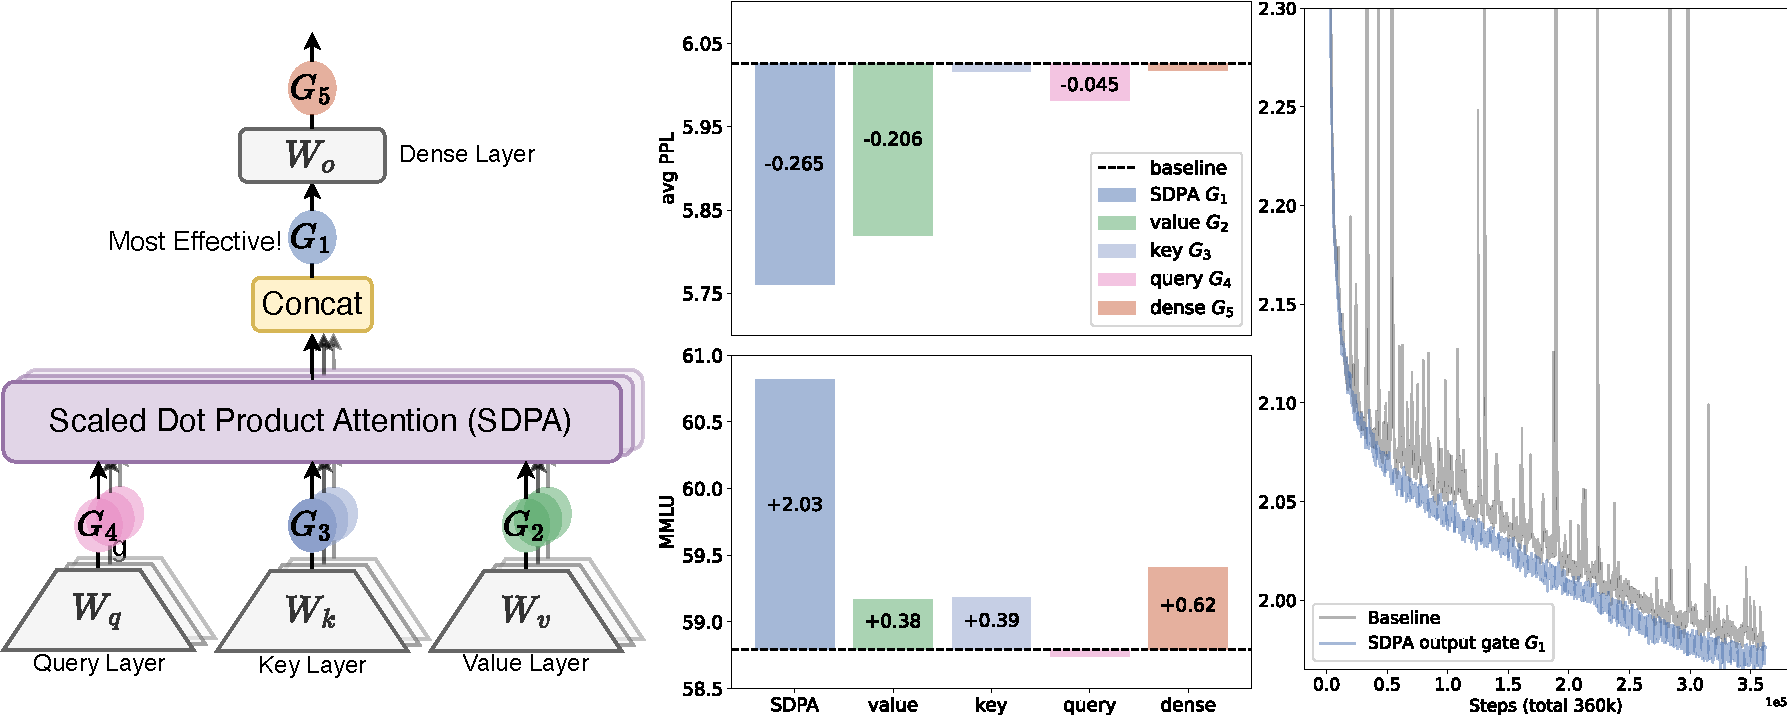
\includegraphics[width=1.0\textwidth]{imgs/gate_results.pdf}
    }
\vskip  -0.05in
  \caption{\footnotesize \textbf{左}：门控操作的候选位置；
  \textbf{中}：15B MoE 模型在不同门控位置下的性能对比（测试 PPL 与 MMLU）。
  在 SDPA 之后门控（$G_1$）总体最佳，Value 层后门控（$G_2$）也有显著提升，尤其在 PPL 上。
  \textbf{右}：在相同超参下，基线与 SDPA 门控的 1.7B 稠密模型在 3.5T tokens 上的训练损失对比（平滑系数 0.9）。
  门控带来更低的最终损失并显著提升训练稳定性，缓解损失尖峰。
  这种稳定性允许更高学习率并促进更好的尺度扩展。
  }
  \label{fig:gate_results}
  \end{center}
  \vskip  -0.3in
\end{figure*}




\section{门控注意力层}

\subsection{预备：多头 Softmax 注意力}

给定输入 $ X \in \mathbb{R}^{n \times d_{\text{model}}} $，其中 $ n $ 为序列长度，$ d_{\text{model}} $ 为模型维度，Transformer 的注意力层~\citep{vaswani2017attention} 计算可分为四个阶段。

\paragraph{QKV 线性投影：} 输入 $ X $ 通过可学习权重矩阵 $ W_Q, W_K, W_V \in \mathbb{R}^{d_{\text{model}} \times d_k}$ 线性变换为查询 $ Q $、键 $ K $ 与值 $ V $，其中 $ Q, K, V \in \mathbb{R}^{n \times d_k}$：
\begin{equation}
Q = XW_Q, \quad K = XW_K, \quad V = XW_V.
\label{eq:qkv_map}
\end{equation}

\paragraph{缩放点积注意力（SDPA）：} 计算查询与键的注意力分数，并进行 softmax 归一化。输出为 value 的加权求和：
\begin{equation}
   \text{Attention}(Q, K, V) = \text{softmax}\left(\frac{QK^T}{\sqrt{d_k}}\right)V,
\end{equation}
其中 $ \frac{QK^T}{\sqrt{d_k}} \in \mathbb{R}^{n \times n} $ 为缩放点积相似度矩阵，$ \text{softmax}(\cdot) $ 保证注意力权重非负并在每行求和为 1。

\paragraph{多头拼接：} 在多头注意力中，上述过程对 $ h $ 个头并行执行，每个头拥有其投影矩阵 $ W_q^i, W_k^i, W_v^i $。所有头的输出被拼接：
\begin{equation}
   \text{MultiHead}(Q, K, V) = \text{Concat}(\text{head}_1, \dots, \text{head}_h),
\label{eq:SDPA}
\end{equation}
其中 $ \text{head}_i = \text{Attention}(QW_Q^i, KW_K^i, VW_V^i) $。

\paragraph{最终输出层：} 拼接后的 SDPA 输出通过输出层 $ W_o \in \mathbb{R}^{h d_k \times d_{\text{model}}}$：
\begin{equation}
   O = \text{MultiHead}(Q, K, V)W_o.
\label{eq:output}
\end{equation}

\begin{figure*}[t!]
    \vskip  -0.3in
    \begin{center}\centerline{
    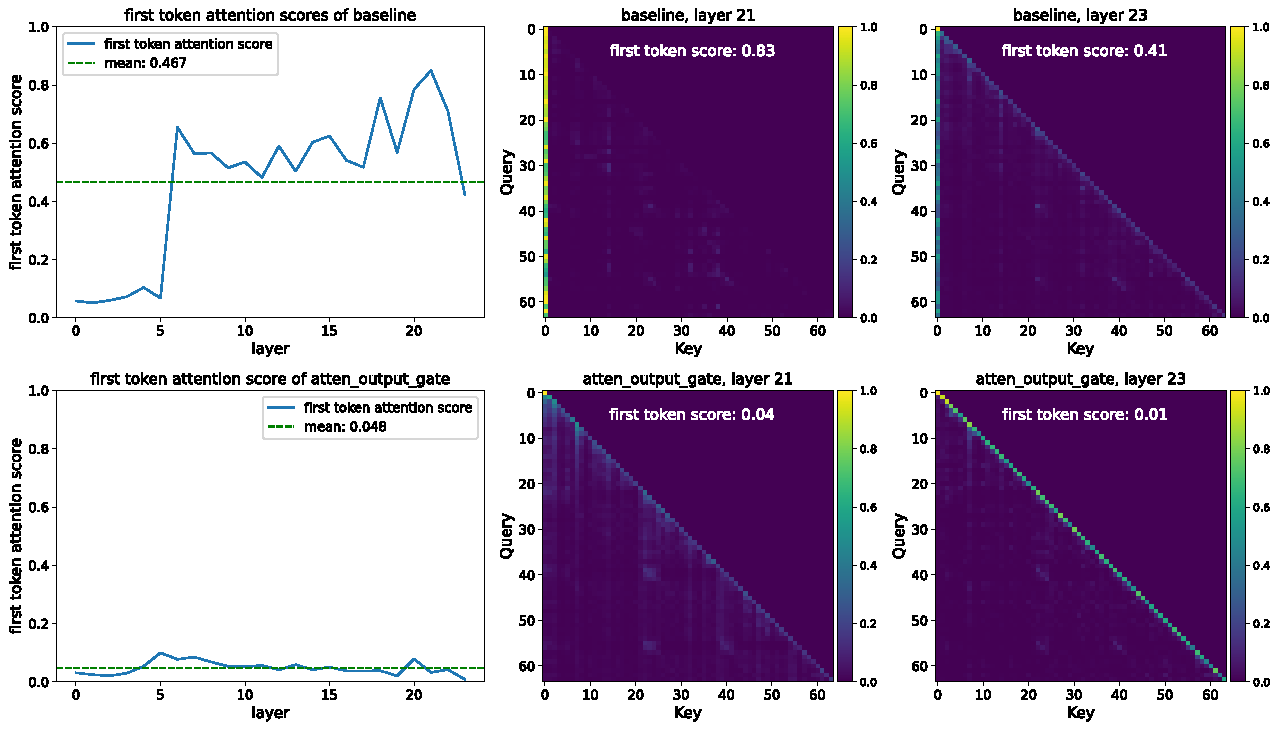
\includegraphics[width=1.0\textwidth]{imgs/attn_scores.pdf}
    }
\vskip  -0.1in
  \caption{\footnotesize \textbf{左}：每层分配给初始 token 的注意力比例（测试困惑度数据集）。基线模型存在显著 attention sink，跨层平均 46.7\% 的注意力分数指向首 token。引入门控后该比例降至 4.8\%。
  \textbf{右}：各头平均注意力图权重。基线模型第 21 层 attention sink 很强（首 token 占 83\%），门控后显著降低（4\%）。
  在最终输出层，门控放大了模型对序列中个别 token 的既有关注倾向。
  }
  \label{fig:attn_results}
  \end{center}
  \vskip  -0.3in
\end{figure*}

\subsection{注意力层的门控增强}
\label{sec:gating_variants}

门控机制形式化为：
\begin{equation}
    Y'= g(Y, X, W_\theta, \sigma) = Y \odot \sigma(X W_\theta),
\label{eq:gate}
\end{equation}
其中 $ Y $ 为待调制输入，$ X $ 为用于计算门控分数的另一输入\footnote{我们将 pre-norm 后的隐藏状态作为 $X$。}，$ W_\theta $ 为门控可学习参数，$ \sigma $ 为激活函数（如 sigmoid），$ Y' $ 为门控输出。
门控分数 $\sigma(X W_\theta)$ 充当动态滤波器，通过选择性保留或抹除特征来控制 $Y$ 的信息流。

本文在注意力层内系统考察多种门控机制变体。
我们的探索聚焦五个关键维度：
\textbf{(1) 位置。}
我们研究在不同位置施加门控的效果，如图~\ref{fig:gate_results}(左) 所示：
(a) 在 $Q, K, V$ 投影（式~\ref{eq:qkv_map}）之后，对应图中的 $G_2, G_3, G_4$；
(b) 在 SDPA（式~\ref{eq:SDPA}）输出之后（$G_1$）；
(c) 在最终多头拼接输出之后（式~\ref{eq:output}，$G_5$）。
\textbf{(2) 粒度。}
我们考虑两种门控分数粒度：(a) 按头：单个标量门控分数调制整个注意力头输出；
(b) 元素级：门控分数为与 $Y$ 同维的向量，可进行逐维细粒度调制。
\textbf{(3) 头部特异或共享。}
考虑到多头结构，我们进一步区分：(a) 头部特异：每个注意力头拥有独立门控分数；
(b) 头部共享：$W_\theta$ 与门控分数在所有头之间共享。
\textbf{(4) 乘性或加性。}
门控分数应用到 $Y$ 的方式包括：(a) 乘性门控：$Y' = Y \cdot \sigma(X\theta)$；
(b) 加性门控：$Y' = Y + \sigma(X\theta)$。
\textbf{(5) 激活函数。}
我们主要考虑 SiLU~\citep{shazeer2020glu} 与 sigmoid 两种常见激活。
由于 SiLU 输出无界，我们仅用于加性门控；sigmoid 仅给出 $[0,1]$ 分数。
此外，为进一步剖析门控有效性的机制，我们还考虑恒等映射或 RMSNorm~\citep{zhang2019root}（详见第~\ref{sec:non-linearity} 节）。

除非另有说明，我们使用按头特异的乘性门控，并采用 sigmoid 激活（$ \sigma(x) = \frac{1}{1 + e^{-x}} $）。
% , to study the impact of gating positions.
% We then compare the effects of various gating variants, identify the most effective gatings, and uncover the reasons for their success.


\section{实验}



\subsection{实验设置}

\paragraph{模型架构与训练设置} 
我们在 MoE 模型（总参数 15B、激活 2.54B，15A2B）与稠密模型（总参数 1.7B）上进行实验。
15A2B MoE 模型采用 128 个专家、top-8 softmax 门控、细粒度专家~\citep{dai2024deepseekmoe}、全局批次 LBL~\citep{global_balance} 与 z-loss~\citep{zoph2022st}。
注意力部分采用 GQA~\citep{ainslie2023gqa}。
我们在 3.5T 高质量 token 的子集上训练模型，覆盖多语言、数学与通用知识内容。
上下文长度设为 4096。
更详细的配置（如学习率与 batch size）将在各小节中说明。
其他超参数采用 AdamW 默认设置。
由于门控引入的参数与 FLOPs 较小，\textit{门控带来的墙钟时延低于 2\%。}

\paragraph{评测} 我们在常用基准上测试 few-shot 结果，包括：英文 Hellaswag~\citep{zellers2019hellaswag}、通用知识 MMLU~\citep{hendrycks2020measuring}、数学推理 GSM8k~\citep{cobbe2021training}、代码 HumanEval~\citep{chen2021codex}、中文能力 C-eval~\citep{huang2024c} 与 CMMLU~\citep{li2023cmmlu}。
我们还在多种保留测试集上报告语言建模困惑度（PPL），覆盖英文、中文、代码、数学、法律与文学等领域。


\begin{table}[t!]
\centering
\vskip  -0.25in
\caption{\footnotesize 门控变体的性能与结果。
我们在 \textbf{400B} tokens 上训练 \textbf{15A2B} MoE 模型。
$d_k$ 为头维度，$d_{\text{model}}$ 为模型隐藏维度，$n$ 为 token 数。
$q$ 表示 query 头数，$k$ 表示 key-value 头数。`Act Func` 为式~\ref{eq:gate} 中的激活函数，`Score Shape` 为输入 $X \in \mathbb{R}^{n, d_{\text{model}}}$ 的门控分数形状。
`added param` 表示新增参数量（百万）。}
\vskip  -0.1in
\label{tab:gating-methods}
\resizebox{\textwidth}{!}{
\begin{tabular}{lccc|ccccc}
\toprule
\textbf{方法} & \textbf{激活函数} & \textbf{分数形状}  & \textbf{新增参数} & \textbf{平均 PPL} & \textbf{Hellaswag} & \textbf{MMLU} & \textbf{GSM8k} & \textbf{C-eval} \\
\midrule
\multicolumn{9}{c}{参考基线（基线使用 $q=32, k=4$，所有方法 $d_k=128$）} \\
\midrule
(1) Baseline & - & - & 0 & 6.026 & 73.07 & 58.79 & 52.92 & 60.26 \\
(2) $k=8$ & - & - & 50 & 5.979 & 73.51 & 59.78 & 52.16 & 62.26 \\
(3) $q=48$ & - & - & 201 & 5.953 & 73.59 & 58.45 & 53.30 & 59.67 \\
(4) Add 4 Experts & - & - & 400 & 5.964 & 73.19 & 58.84 & 52.54 & \textbf{63.19} \\
\midrule
\multicolumn{9}{c}{门控位置变体} \\
\midrule
(5) SDPA Elementwise $G_1$ & sigmoid & $n\times q \times d_k$ & 201 & \textbf{5.761} & 74.64 & \textbf{60.82} & \textbf{55.27} & 62.20 \\
(6) v Elementwise $G_2$  & sigmoid & $n\times k \times d_k$ & 25 & 5.820 & 74.38 & 59.17 & 53.97 & 61.00 \\
(7) k Elementwise $G_3$  & sigmoid & $n\times k \times d_k$ & 25 & 6.016 & 72.88 & 59.18 & 50.49 & 61.74 \\
(8) q Elementwise $G_4$ & sigmoid & $n\times q \times d_k$ & 201 & 5.981 & 73.01 & 58.74 & 53.97 & 62.14 \\
(9) Dense Output $G_5$  & sigmoid & $n \times d_{\text{model}}$ & 100 & 6.017 & 73.32 & 59.41 & 50.87 & 59.43 \\
\midrule
\multicolumn{9}{c}{门控粒度变体} \\
\midrule
(10) SDPA Headwise $G_1$ & sigmoid & $n\times q$ & 1.6 & 5.792 &	74.50 & 60.05 & 54.44 & 62.61 \\
(11) v Headwise $G_2$  & sigmoid & $n\times q$ & 0.2 & 5.808	&  74.38 &	59.32 &	53.53 &	62.61 \\
\midrule
\multicolumn{9}{c}{头部特异 vs. 头部共享门控} \\
\midrule
(12) SDPA Head-Shared $G_1$ & sigmoid & $n\times d_k$ & 201 & 5.801 & 74.34 & 60.06 &	53.15	& 61.01 \\
(13) v Head-Shared $G_2$  & sigmoid & $n\times d_k$ &25 & 5.867	&  74.10 &	59.02 &	53.03 &	60.61 \\
\midrule
\multicolumn{9}{c}{乘性 vs. 加性} \\
\midrule
(14) SDPA Additive $G_1$ & SiLU & $n\times q \times d_k$ & 201 & 5.821 & \textbf{74.81} &	60.06 &	53.30 &	60.98\\
\midrule
\multicolumn{9}{c}{激活函数变体} \\
\midrule
(15) SDPA Elementwise $G_1$ & SiLU & $n\times q \times d_k$ & 201 & 5.822 & 74.22 &	60.49 &	54.59 &	62.34\\
\bottomrule
\end{tabular}
}
% \vskip  -0.15in
\end{table}


\subsection{主要结果}
\label{sec:main_results}

\subsubsection{MoE 模型的门控注意力}
\label{sec:MoE-exp}

我们首先在训练效率更高的 MoE-15A2B 模型上对比不同门控注意力层的结果。
所有模型使用学习率调度：1k 步升温至最大 LR=2e-3，并采用余弦衰减至 3e-5。
全局 batch size 为 1024，总计 100k 步优化。
结果汇总于表~\ref{tab:gating-methods}。
为公平比较，我们在原始 MoE 基线（第 1 行）之外加入参数扩展方法，包括增加 key-value 头数（第 2 行）、增加 query 头数（第 3 行）、以及同时增加专家总数与激活专家数（第 4 行）。
这些方法引入的参数量与门控机制相当或更高。




从表~\ref{tab:gating-methods} 可观察到：
\textbf{(i) SDPA 与 value 输出门控有效。} 在 SDPA 输出（$G_1$）或 value 映射（$G_2$）处加入门控最有效，相比其他变体获得更低 PPL 与更高综合基准表现。
我们将在第~\ref{sec:sparsity} 节进一步分析为何这两个位置有效。
\textbf{(ii) 头部特异门控很重要。} 在 $G_1$ 与 $G_2$ 施加按头门控仅引入极少参数（MoE-15A2B 少于 2M），却仍带来显著提升（第 10、11 行）。
若在不同注意力头之间共享门控分数（将原始 $n \times q \times d_k$ 在 query 头维度 $q$ 上平均，得到 $n \times d_k$），其基准提升小于按头门控（第 12 vs. 10 行、13 vs. 11 行），强调了对不同注意力头使用不同门控分数的重要性。
\textbf{(iii) 更偏好乘性门控。} SDPA 输出的加性门控虽优于基线，但弱于乘性门控。
\textbf{(iv) Sigmoid 更优。} 将最有效门控配置（第 5 行）的激活由 sigmoid 换为 SiLU（第 15 行）会带来更小的提升。

总体而言，在 value 层（$G_2$）与 SDPA 输出（$G_1$）加入门控可使 PPL 降低超过 0.2，优于多种参数扩展基线。
其中 $G_1$ 的门控在 PPL 与基准成绩上更好。
只要不同头拥有不同门控分数，门控粒度与激活函数的选择影响相对较小。
我们将在分析部分（第~\ref{sec:sparsity} 节）进一步解释这些现象。


\subsubsection{稠密模型的门控注意力}
\label{sec:dense-exp}


我们还按照~\citep{yang2024qwen2} 在稠密模型上进行实验以验证 SDPA 输出的 sigmoid 门控。
使用门控时，我们适当缩小 FFN 宽度以保持参数规模一致。
多数实验使用基线的优化超参。
例如，1.7B 模型在 400B tokens 上训练时使用最大 LR 4e-3、bsz 1024；在 3.5T tokens 上训练时将最大 LR 提升到 4.5e-3、bsz 提升到 2048。
已有工作指出，增加网络深度、较大学习率与较大 batch size 可显著提升模型性能~\citep{mccandlish2018empirical, wang2022deepnetscalingtransformers1000, d2024we} 与分布式训练效率，但也常引入训练不稳定~\citep{wang2022deepnetscalingtransformers1000,zeng2022glm, takase2023spike}。
我们观察到门控机制能显著降低训练中的损失尖峰~\citep{chowdhery2023palm, takase2023spike}，提示其有望增强训练稳定性。
基于此，我们引入另一组实验设置：增加层数、提高最大学习率、增大 batch size，以进一步验证门控的稳定化作用。

\begin{table}[t!]
\centering
\vskip  -0.2in
\caption{\footnotesize 不同学习率、batch size 与模型配置下的方法性能。
`SDPA` 指式~\ref{eq:SDPA} 中 SDPA 后的 sigmoid 门控，`sandwitch norm`~\citep{ding2021cogview} 表示在加入残差前对 attention/FFN 输出进行归一化。
使用门控时我们缩小 FFN 宽度以保持参数量一致。`-` 表示训练发散。}
\vskip  -0.1in
\label{tab:data-lr-variants}
\resizebox{\textwidth}{!}{
\begin{tabular}{lc|ccccccc}
\toprule
\textbf{Method} & \textbf{Max LR} & \textbf{Avg PPL} & \textbf{HumanEval} & \textbf{MMLU} & \textbf{GSM8k} & \textbf{Hellaswag} & \textbf{C-eval} & \textbf{CMMLU} \\
\midrule
\multicolumn{9}{c}{28 Layer, 1.7B Parameters, \textbf{400B Tokens}, Batch Size=1024} \\
\midrule
(1) Baseline & $4.0 \times 10^{-3}$ & 7.499 & 28.66 & 50.21 & 27.82 & 64.94 & 49.15 & 49.52 \\
(2) SDPA Elementwise & $4.0 \times 10^{-3}$ & \textbf{7.404} & \textbf{29.27} & \textbf{51.15} & \textbf{28.28} & \textbf{65.48} & \textbf{50.72} & \textbf{50.72} \\
\midrule
\multicolumn{9}{c}{28 Layer, 1.7B Parameters, \textbf{3.5T Tokens}, Batch Size=2048} \\
\midrule
(3) Baseline & $4.5 \times 10^{-3}$ & 6.180 & 34.15 & 59.10 & 69.07 & 68.02 & 68.19 & 64.95 \\
(4) SDPA Elementwise & $4.5 \times 10^{-3}$ & \textbf{6.130} & \textbf{37.80} & \textbf{59.61} & \textbf{70.20} & \textbf{68.84} & \textbf{68.52} & \textbf{65.76} \\
\midrule
\multicolumn{9}{c}{48 Layer, 1.7B Parameters, 
\textbf{400B Tokens}, Batch Size=1024} \\
\midrule
(5) Baseline & $4.0 \times 10^{-3}$ & 7.421 & 28.05 & 52.04 & 32.98 & 65.96 & 51.11 & 51.86 \\
(6) Baseline & $8.0 \times 10^{-3}$ & 9.195 & 21.34 & 44.28 & 15.24 & 57.00 & 43.11 & 42.63 \\
(7) Baseline+Sandwich Norm & $8.0 \times 10^{-3}$ & 7.407 & 30.49 & 52.07 & 32.90 & 66.00 & 52.04 & 51.72 \\
(8) SDPA Elementwise & $4.0 \times 10^{-3}$ & \textbf{7.288} & \textbf{31.71} & 52.44 & 32.37 & 66.28 & 52.06 & 52.29 \\
(9) SDPA Headwise & $4.0 \times 10^{-3}$ & 7.370 & 31.10 & 53.83 & 34.12 & 65.59 & \textbf{55.07} & 52.38 \\
(10) SDPA Elementwise & $8.0 \times 10^{-3}$ & 7.325 & 31.10 & \textbf{54.47} & \textbf{36.62} & \textbf{66.40} & 53.91 & \textbf{53.80} \\
\midrule
\multicolumn{9}{c}{48 Layer, 1.7B Parameters, \textbf{1T Tokens}, Batch Size=4096} \\
\midrule
(11) Baseline & $5.3 \times 10^{-3}$ & 7.363 & 29.88 & 54.44 & 32.22 & 65.43 & 53.72 & 53.37 \\
(12) Baseline & $8.0 \times 10^{-3}$ & - & - & - & - & - & - & - \\
(13) SDPA Elementwise & $5.3 \times 10^{-3}$ & 7.101 & \textbf{34.15} & 55.70 & 36.69 & 67.17 & 54.51 & 54.68 \\
(14) SDPA Elementwise & $8.0 \times 10^{-3}$ & \textbf{7.078} & 31.71 & \textbf{56.47} & \textbf{39.73} & \textbf{67.38} & \textbf{55.52} & \textbf{55.77} \\
\bottomrule
\end{tabular}
}
% \vskip  -0.15in
\end{table}


表~\ref{tab:data-lr-variants} 表明：
\textbf{(i) 门控在多种设置下有效。} 在不同模型配置（第 1 vs. 2 行、5 vs. 8 行）、训练数据规模（第 3 vs. 4 行）与超参（第 11 vs. 13 行）下，SDPA 输出门控均持续带来收益。
\textbf{(ii) 门控提升稳定性并促进扩展。} 在 3.5T tokens 设置下，门控显著提升训练稳定性并大幅减少损失尖峰（图~\ref{fig:gate_results} 右）。
当提高最大 LR 时，基线出现收敛问题（第 6、12 行）；添加 sandwich norm~\citep{ding2021cogview} 可恢复收敛，但提升有限。相反，门控模型提高最大 LR 可获得明显改善。

综上，我们认为 SDPA 元素级门控是增强注意力机制最有效的方法。
将该方法应用于稠密 Transformer 进一步表明：\textit{门控可在更大 batch size 与更高学习率下保持稳定训练，从而带来更好的性能。}


\section{分析：非线性、稀疏性与无注意力汇聚}

本节通过一系列实验解释为何如此简单的门控机制能显著提升性能与训练稳定性。
主要结论如下：
(1) 增强非线性的门控操作稳定带来性能提升（第~\ref{sec:non-linearity} 节）；
(2) 最有效的 SDPA 元素级 $G_1$ 门控为 SDPA 输出引入强烈的输入相关稀疏性（第~\ref{sec:sparsity} 节），从而有助于消除 attention sink 现象。

\subsection{非线性提升注意力中低秩映射的表达能力}
\label{sec:non-linearity}

\begin{table}[t!]
\centering
\vskip  -0.25in
\caption{\footnotesize 不同（非）线性增强方法的性能。}
\vskip  -0.1in
\label{tab:SDPA-activation}
\resizebox{0.85\textwidth}{!}{
\begin{tabular}{lc|ccccc}
\toprule
\textbf{方法} & \textbf{激活函数} & \textbf{平均 PPL} & \textbf{Hellaswag} & \textbf{MMLU} & \textbf{GSM8k} & \textbf{C-eval} \\
\midrule
(1) Baseline & - & 6.026 & 73.07 & 58.79 & 52.92 & 60.26 \\
(2) SDPA Elementwise Gate & Sigmoid & \textbf{5.761} & 74.64 & \textbf{60.82} & \textbf{55.27} & \textbf{62.20} \\
(3) v Elementwise Gate & Sigmoid &  5.820 & 74.38 & 59.17 & 53.97 & 61.00 \\
(4) SDPA Additive Gate & SiLU & 5.821 & \textbf{74.81} & 60.06 & 53.30 & 60.98 \\
\midrule
(5) SDPA GroupNorm & RMSNorm & 5.847 & 74.10 & 60.15 & 53.75 & 61.14 \\
(6) SDPA SiLU & SiLU & 5.975 & 73.34 & 59.55 & 53.19 & 60.90 \\
(7) SDPA Additive Gate & Identity & 5.882 & 74.17 & 59.20 & 52.77 & 59.86 \\
\bottomrule
\end{tabular}
}
% \vskip  -0.15in
\end{table}



受此前在 SDPA 输出上使用 group norm 的工作启发~\citep{sun2023retentivenetworksuccessortransformer,ye2024differential}，在与第~\ref{sec:MoE-exp} 节相同设置下，我们对每个注意力头的输出在拼接前独立应用 RMSNorm~\citep{zhang2019root}。
如表~\ref{tab:SDPA-activation} 第 5 行所示，RMSNorm 几乎不引入额外参数，却能显著降低 PPL。

在多头注意力中，第 $k$ 个头对应的第 $i$ 个 token 输出可表示为：
\begin{align}
o^k_i &= (\sum\nolimits_{j=0}^{i} S^k_{ij}  \cdot X_j W_V^k ) W^k_O = \sum\nolimits_{j=0}^{i} S^k_{ij}  \cdot X_j (W_V^k  W^k_O),
\label{eq:attn}
\end{align}
其中 $W^k_O$ 为输出层 $W_O$ 中对应第 $k$ 个头的参数\footnote{注意：先拼接各头输出再乘 $W_O$ 等价于先将每个头输出分别乘其对应的 $W^k_O$ 再拼接。}。
这里 $S^k_{ij}$ 为第 $k$ 个头中第 $i$ 个 token 对第 $j$ 个 token 的注意力分数，$X_j$ 为第 $j$ 个 token 的注意力输入，$X_j W_V^k$ 为该 token 在第 $k$ 个头上的 value 输出。
由式~\ref{eq:attn} 可知，\textit{由于 $d_k < d_{\text{model}}$，可将 $W_V^k W^k_O$ 合并为对所有 $X_j$ 的一个低秩线性映射}。
在 GQA 中，$W_V$ 在同组头之间共享，进一步降低表达能力。


鉴于在线性映射之间加入非线性可提升表达能力~\citep{montufar2014numberlinearregionsdeep}，我们提出两种缓解低秩问题的改动：
\begin{equation}
o^k_i = \left(\sum\nolimits_{j=0}^{i} S^k_{ij}  \cdot \text{Non-Linearity-Map}(X_j W_V^k) \right) W^k_O,
\label{eq:v_non_linearity}
\end{equation}
\begin{equation}
o^k_i = \text{Non-Linearity-Map}\left(\sum\nolimits_{j=0}^{i} S^k_{ij}  \cdot X_j W_V^k \right) W^k_O.
\label{eq:SDPA_non_linearity}
\end{equation}
需要注意的是，在 $G_2$ 处加入门控（表~\ref{tab:SDPA-activation} 第 3 行）对应第一种改动（式~\ref{eq:v_non_linearity}），而在 $G_1$ 处加入门控（第 4 行）或 group normalization（第 5 行）对应第二种改动（式~\ref{eq:SDPA_non_linearity}）。
这也解释了为何在 $W_O$ 之后的 $G_5$ 位置添加门控或归一化无效（表~\ref{tab:gating-methods} 第 9 行）——它并未解决 $W_V$ 与 $W_O$ 之间缺乏非线性的问题。


在 $G_1$ 处的加性门控中，门控输出经过 SiLU（表~\ref{tab:SDPA-activation} 第 4 行），同样引入一定非线性，因此带来性能提升，但弱于乘性门控。
基于此我们进行两项额外实验：\textbf{(i)} 仅在 $G_1$ 位置加入 SiLU 而不引入额外参数（表~\ref{tab:SDPA-activation} 第 6 行）。该简单改动也能小幅降低 PPL，但多数基准分数基本不变。
\textbf{(ii)} 去掉加性门控中的 SiLU，使门控后的 $X_j$ 输出直接在 $G_1$ 位置相加（表~\ref{tab:SDPA-activation} 第 7 行）。
这会进一步削弱加性门控的增益。

综上，有效门控变体带来的性能提升很可能源于在 $W_V$ 与 $W_O$ 之间引入非线性。
尽管在 $G_1$ 与 $G_2$ 位置都可引入非线性，但其性能提升幅度不同。
这一差异促使我们进一步分析这两个位置门控的影响。



\subsection{门控引入与输入相关的稀疏性}
\label{sec:sparsity}

我们在测试语言建模数据上分析了在 value（$G_2$）与 SDPA 输出（$G_1$）位置门控的分数（表~\ref{tab:gating-methods} 中 `Gate Score` 列）。
所有层的门控分数均值见表~\ref{tab:SDPA-gate-score}，分布见图~\ref{fig:gating_scores}（分层分数见附录~\ref{App:sparsity}）。
关键观察包括：

\textbf{(i) 有效门控分数是稀疏的。} SDPA 输出门控（元素级/按头）的平均门控分数最低。
同时，SDPA 输出门控分数的分布高度集中在 0 附近，表明稀疏性很强，与其更优性能一致。
\textbf{(ii) 头部特异的稀疏性很重要。} 若强制在注意力头之间共享门控分数，会提高总体门控分数并削弱性能增益。
观察 (i) 与 (ii) 强调了\textit{头部特异门控}的重要性，这与以往研究一致，即不同注意力头捕获输入的不同方面~\citep{voita2019analyzing, wang2021spatten, olsson2022context,wang2023smarttrim}。

\begin{table}
\centering
\vskip  -0.25in
\caption{\footnotesize 不同门控方法在不同激活函数与平均门控分数下的性能。`Act-Func` 为计算门控分数的激活函数，`M-Act` 表示模型各层输出隐藏状态的最大激活值（取整）。此外，`F-Attn` 为首 token 的注意力分数，值越高表示 attention sink 越明显。}
\vskip  -0.1in
\label{tab:SDPA-gate-score}
\resizebox{\textwidth}{!}{
\begin{tabular}{lcc|cc|cccc}
\toprule
\textbf{方法} & \textbf{激活函数} & \textbf{门控分数} & \textbf{M-Act} & \textbf{F-Attn} & \textbf{PPL} & \textbf{Hellaswag} & \textbf{MMLU} & \textbf{GSM8k} \\
\midrule
(1) Baseline & - & - & 1053 & 0.467 & 6.026 & 73.07 & 58.79 & 52.92 \\
(2) SDPA Elementwise Gate & Sigmoid   & 0.116 & 94 & 0.048 & \textbf{5.761} & \textbf{74.64} & \textbf{60.82} & \textbf{55.27} \\
(3) SDPA Headwise Gate  & Sigmoid   & 0.172 & 98 & 0.073 & 5.792 & 74.50 & 60.05 & 54.44 \\
\midrule
(4) SDPA Elementwise Head-shared Gate & Sigmoid  & 0.271 & 286 & 0.301 & 5.801 & 74.34 & 60.06 & 53.15 \\
\midrule
(5) v Elementwise Gate & Sigmoid  & 0.221 & 125 & 0.297 & 5.820 & 74.38 & 59.17 & 51.33 \\
(6) SDPA Input Independent Gate  & Sigmoid & 0.335 & 471 & 0.364 & 5.917 & 73.64 & 59.02 & 52.40 \\
\midrule
(7) SDPA Elementwise Gate & NS-sigmoid & 0.653 & 892 & 0.451 & 5.900 & 74.05 & 60.05 & 52.75 \\
\bottomrule
\end{tabular}
}
\end{table}

\begin{figure*}[t]
    \vskip -0.15in  \begin{center}\centerline{
    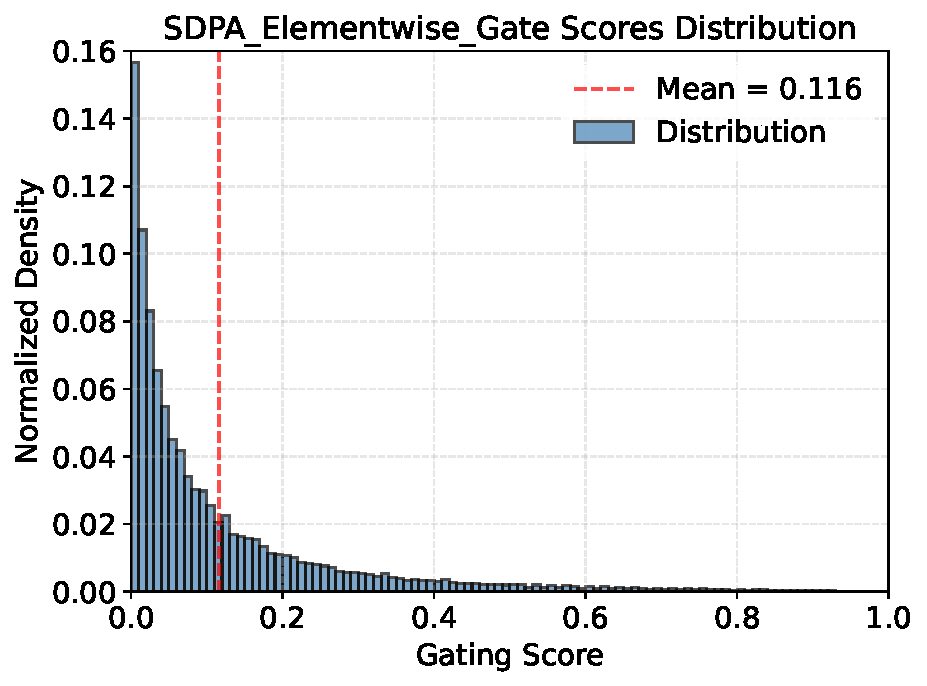
\includegraphics[width=0.33\textwidth]{imgs/SDPA_Elementwise_Gate_distribution.pdf}
    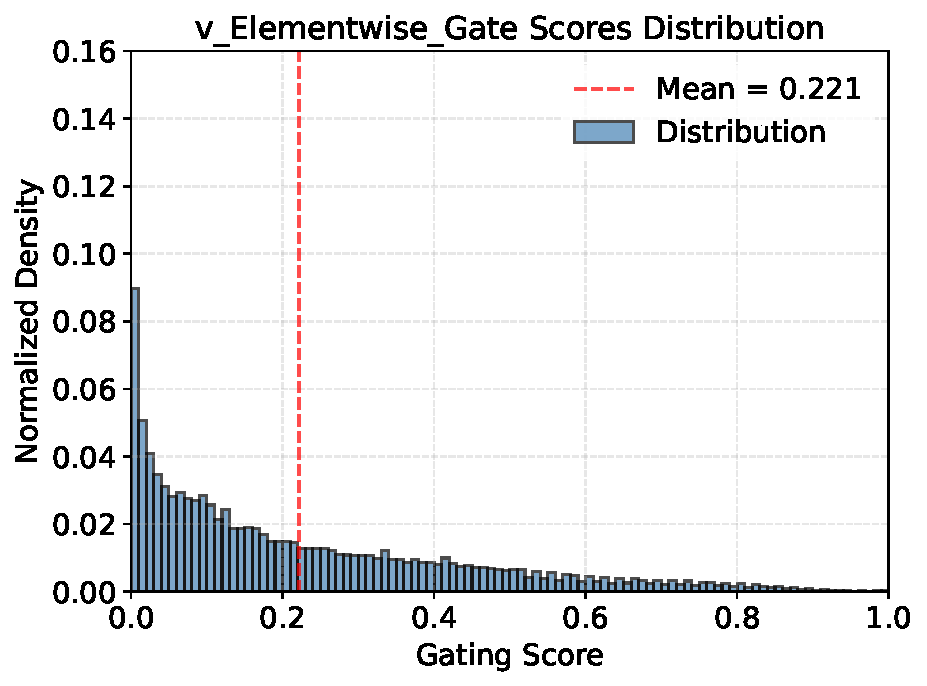
\includegraphics[width=0.33\textwidth]{imgs/v_Elementwise_Gate_distribution.pdf}
    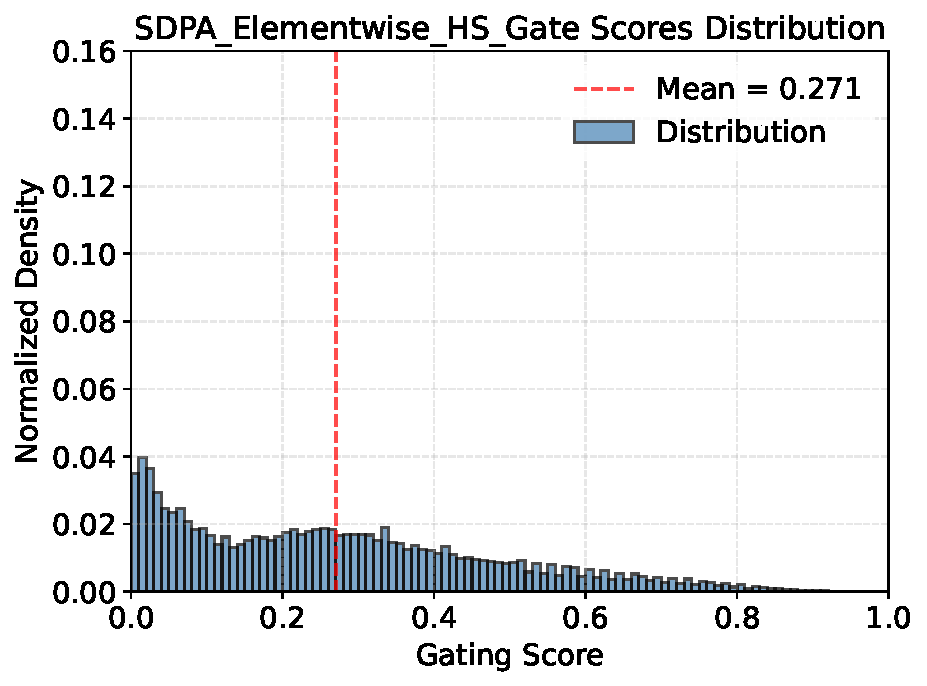
\includegraphics[width=0.33\textwidth]{imgs/SDPA_Elementwise_HS_Gate_distribution.pdf}
    }
\vskip  -0.15in
  \caption{\footnotesize SDPA 元素级（左）、value 元素级（中）以及 SDPA 元素级头部共享（右）的门控分数均值与分布。
多数门控分数小于 0.5，表明门控分数较为稀疏。
其中 SDPA 输出门控的稀疏性最强。
  }
  \label{fig:gating_scores}
  \end{center}
  \vskip  -0.3in
\end{figure*}


\textbf{(iii) Query 相关性很重要。} value 门控（$G_2$）的分数高于 SDPA 输出门控（$G_1$），且性能更差。
这表明门控分数的稀疏性在 query 相关时更有效，而非由 key/value 决定。
具体来说，SDPA 输出门控分数来自当前 query 的隐藏状态（例如式~\ref{eq:SDPA_non_linearity} 中的 Non-Linearity-Map 依赖 $X_i$），而 value 门控分数来自与过去 key/value 关联的隐藏状态（如式~\ref{eq:v_non_linearity} 中依赖各个 $X_j$）。
这意味着\textit{门控分数的稀疏性可能在为 query 过滤无关上下文信息}。
为验证 query 相关性的重要性，我们引入输入无关门控：将可学习参数（$q \times d_k$）初始化为零，经 sigmoid 后与 SDPA 输出相乘。
如第 (6) 行所示，输入无关门控相较基线有所提升，可能来自非线性的引入。
同时，高门控分数进一步说明有效稀疏性应当是输入相关的。


% [t!]
\textbf{(iv) 稀疏性降低会变差。} 为进一步验证门控稀疏性的关键作用，我们削弱门控公式中的稀疏性，具体用非稀疏（NS）版本替代 sigmoid：
$$
\text{NS-sigmoid}(x) = 0.5 + 0.5 \cdot \text{sigmoid}(x),
$$  
which constrains the gating scores between [0.5, 1.0]. 
该方式保留非线性但移除门控分数的稀疏性。
如表~\ref{tab:SDPA-gate-score} 第 (7) 行所示，NS-sigmoid 门控的收益低于 SDPA 输出 sigmoid 门控。
在附录~\ref{App:sparsity} 中，我们进一步讨论稀疏门控分数如何影响 SDPA 隐状态的稀疏性（低于阈值的比例）。
下一节我们将讨论不同稀疏程度对模型行为的影响，包括减少 attention sink。

\subsection{SDPA 输出门控减少 Attention-Sink}
\label{sec:sink}

基于门控以输入相关方式为 SDPA 输出引入稀疏性的观察，我们假设该机制能过滤当前 query token 无关的上下文，从而缓解 attention sink~\citep{xiao2023efficient, sun2024massive}。
为验证这一点，我们分析注意力分数分布（对所有头取平均）以及分配给首 token 的注意力分数比例（图~\ref{fig:attn_results}，表~\ref{tab:SDPA-gate-score} 中 `F-Attn` 列）。
受关于隐藏状态巨大激活与 attention sink 的讨论启发~\citep{sun2024massive}，我们还计算各层最大隐藏状态激活的平均值，如表~\ref{tab:SDPA-gate-score} 的 `M-Act` 列所示。
更详细的分层结果见附录~\ref{app:massive-sink}。

我们观察到：
\textbf{(i)} 在 SDPA 输出（$G_1$）处施加按头或元素级、与 query 相关的 sigmoid 门控，会显著降低分配给首 token 的注意力分数，并减小巨大激活。
\textbf{(ii)} 若在头之间共享门控分数，或仅在 value 投影后施加门控（$G_2$），虽然巨大激活会下降，但首 token 的注意力分数并未降低。这进一步强调头部特异门控的重要性，并表明\textit{巨大激活并非 attention sink 的必要条件}。
\textbf{(iii)} 降低门控的输入相关性（第 6 行）或使用 NS-sigmoid 减少稀疏性（第 7 行）会加剧巨大激活与 attention sink。

综合来看，这些观察表明\textit{在 SDPA 输出处施加输入相关、头部特异的门控会引入显著稀疏性，从而缓解 attention sink。}
此外，SDPA 输出的稀疏性会减少模型内部的巨大激活，且稀疏性越强，激活越小。
\textit{这可能解释了门控带来的训练稳定性提升：通过减少巨大激活，模型在 BF16 训练中更不易出现数值错误~\citep{budzinskiy2025numerical}。}
我们还观察到巨大激活主要来源于早期层（如第 5 层）的 FFN 输出，这与~\citep{yona2025interpreting} 一致。
当这些激活加入残差流后，会通过 pre-norm 机制传播到后续层。这与 sandwich normalization~\citep{ding2021cogview} 在提升训练稳定性方面的有效性一致（表~\ref{tab:data-lr-variants} 第 7 行）：对 FFN 输出施加 LayerNorm 可阻止巨大激活进入残差流。

\subsection{SDPA 输出门控促进上下文长度扩展}
\label{sec:context_extension}

\begin{wraptable}{r}{0.7\textwidth}
\centering
\vskip  -0.15in
\caption{\footnotesize 不同方法在不同序列长度下的性能。`YaRN Extended` 表示扩展上下文长度的变体。
`(数值)` 表示扩展上下文长度后的性能下降幅度。}
\vskip  -0.1in
\label{tab:sequence-length-performance}
\resizebox{0.7\textwidth}{!}{
\begin{tabular}{l|cccccc}
\toprule
\textbf{Method} & \textbf{4k} & \textbf{8k} & \textbf{16k} & \textbf{32k} & \textbf{64k} & \textbf{128k} \\
\midrule
Baseline & 88.89 & 85.88 & 83.15 & 79.50 & - & - \\
SDPA-Gate & 90.56 & 87.11 & 84.61 & 79.77 & - & - \\
\midrule
\multicolumn{7}{c}{YaRN Extended} \\
\midrule
Baseline & 82.90(-6.0) & 71.52(-14.4) & 61.23(-21.9) & 37.94(-41.56) & 37.51 & 31.65 \\
SDPA-Gate & 88.13(-2.4) & 80.01(-7.1) & 76.74(-7.87) & 72.88(-6.89) & 66.60 & 58.82 \\
\bottomrule
\end{tabular}
}
\vskip  -0.15in
\end{wraptable}


基于无 attention sink 的模式，我们评估 SDPA 门控在长上下文场景下的影响。
具体而言，我们对在 3.5T tokens 上训练的模型扩展上下文长度。
我们将 RoPE~\citep{su2024roformer} 基数从 10k 提升到 1M，并继续在 32k 序列长度的数据上训练额外 80B tokens。
由此获得上下文长度为 32k 的模型。
随后使用 YaRN~\citep{peng2023yarn} 将上下文长度扩展至 128k。
我们在 RULER 基准~\citep{hsieh2024ruler} 上评估模型，并在表~\ref{tab:sequence-length-performance} 中汇总结果。
观察如下：
\textbf{(i)} 在 32k 设置下，门控模型略优于基线。
这表明在训练长度内，attention sink 现象可能未显著损害模型的长上下文性能。
\textbf{(ii)} 使用 YaRN 将上下文扩展至 128k 后，基线与门控模型在原始 32k 范围内均出现性能下降。
该现象与通过修改 RoPE 扩展上下文的先前工作一致~\citep{chen2023extendingcontextwindowlarge,peng2023yarn,Dong2025LongReDMS}，但门控模型下降更小。
\textbf{(iii)} 在 64k 与 128k 上下文长度下，门控注意力模型显著优于基线。
基于这些观察，我们推测门控有助于模型适应上下文长度扩展。
一个可能解释是：基线模型依赖 attention sink 来调整注意力分数分布。
~\citet{Dong2025LongReDMS} 从注意力与隐藏状态分布推导了 RoPE 变化的影响。
当像 YaRN 这样的技术改变 RoPE 基数时，attention sink 模式可能难以在无训练的条件下适应，导致明显性能下降。
相反，门控模型主要依赖输入相关的门控分数来控制信息流，因此对这类变化更鲁棒。


\section{相关工作}

\subsection{神经网络中的门控}

门控机制在神经网络中被广泛采用。早期工作如 LSTM~\citep{hochreiter1997long} 与 GRU~\citep{dey2017gate} 通过门控调节跨时间步的信息流，借由选择性保留或丢弃信息来缓解梯度消失/爆炸问题。
Highway Networks~\citep{srivastava2015highway} 将该思想扩展到前馈网络，使得超深架构可被有效训练。
SwiGLU~\citep{shazeer2020glu} 将门控引入 Transformer 的 FFN 层，增强表达能力，并成为许多开源 LLM 的标准组件~\citep{grattafiori2024llama, yang2024qwen2}。


关于状态空间模型~\citep{gu2023mamba,mamba2} 与线性注意力的若干工作（如 FLASH~\citep{hua2022transformer}、RetNet~\citep{sun2023retentivenetworksuccessortransformer}、Lightning Attention~\citep{qin2024lightning, qin2024various, li2025minimax}、Gated Delta Networks~\citep{yang2024gated}）也引入门控模块来调制 token-mixer 的信息流。
Forgetting Transformer~\citep{lin2025forgetting} 将门控应用于 softmax 注意力输出并观察到显著性能提升。
尽管这些工作展示了门控的有效性，但对其精确机制及其有效性原因的系统理解仍有待进一步探索。
这将有助于超越 RNN 范式更全面地认识门控的重要性，并推动更好地利用门控独特优势的设计。
例如，Switch Heads~\citep{csordas2024switchhead, csordas2024moeut}、NSA~\citep{yuan2025native} 与 MoSA~\citep{piękos2025mixturesparseattentioncontentbased} 使用基于 sigmoid 的门控~\citep{csordas2023approximating} 进行选择，若进一步隔离门控的具体贡献，可能带来更有价值的洞见。
与标准 Transformer 中加入类似门控机制的基线进行对比，也能更精细地理解其选择机制的有效性。
与我们最相关的工作是 Quantizable Transformers~\citep{bondarenko2023quantizable}，其同样发现在 softmax 注意力中加入门控可缓解 BERT 与 ViT 等编码器模型中的极端注意力集中与隐藏状态离群值。
该工作主要利用门控消除离群值以便量化，而我们对多种门控变体进行了细致分析，揭示其通过引入非线性与稀疏性、以及改善训练稳定性而带来的收益。
在此基础上，我们将门控注意力扩展到更大规模，展示其广泛适用性与影响力。

\subsection{Attention Sink}

\citet{xiao2023efficient} 正式提出了 “attention sink” 现象，即某些特定 token 获得过大的注意力分数。
类似地，\citet{darcet2023vision} 在视觉 Transformer 中发现，一些冗余 token 充当“寄存器”以存储注意力分数。
随后，\citet{sun2024massive} 指出过大的注意力分数也与巨大激活值相关联的 token 相对应。
然而，我们的工作发现：在 value 投影输出处加入门控可消除巨大激活，但 attention sink 仍可能存在，表明巨大激活并非 attention sink 的必要条件。
同样，\citet{gu2024attention} 将 attention sink 描述为存储冗余注意力分数的非信息性“key bias”，并认为 softmax 的归一化依赖性驱动了该行为。
一些修改 softmax 注意力的实验尝试（如用未归一化的 sigmoid 注意力替代 softmax~\citep{ramapuram2024theory, gu2024attention}，添加 softmax 注意力门控或裁剪~\citep{bondarenko2023quantizable}，以及修改 softmax 计算~\citep{zuhri2025softpickattentionsinkmassive} 与分母~\citep{miller2023offone}）显示出缓解 attention sink 的潜力。
我们的工作表明，在 SDPA 后施加稀疏门控可在稠密（1B 参数）与 MoE（15B 参数）模型中消除 attention sink，即便模型训练于 3.5T tokens。
此外，我们揭示了消除 attention sink 有助于上下文长度扩展。

\section{结论}

本文系统研究了标准 softmax 注意力中的门控机制，揭示其对性能、训练稳定性与注意力动态的显著影响。
通过对训练于最多 3.5T tokens 的 15B MoE 与 1.7B 稠密模型共 30 种变体进行广泛比较，我们证明在缩放点积注意力后施加 sigmoid 门控带来最显著的提升。
该简单机制增强非线性、引入与输入相关的稀疏性，并消除如 attention sink 等低效现象。
此外，门控促进上下文长度扩展，使模型无需再训练即可有效泛化到更长序列。
我们还发布了首批无 attention sink 的模型。
我们相信这些实证结果将为下一代先进基础模型的工程化奠定基础。




\section*{局限性}

我们的工作主要通过一系列消融实验分析注意力门控的原因与影响。
但仍存在若干局限。
非线性对注意力动态与整体训练过程的更广泛影响仍缺乏深入探索。
尽管我们观察到消除 attention sink 可改善长上下文扩展场景的性能，但尚未给出严格的理论解释说明 attention sink 如何影响模型对更长序列的泛化能力。

\bibliography{custom}
\bibliographystyle{colm2024_conference}

\appendix

\section{补充实验}



\subsection{Switch Head 基线}
\label{sec:switch}

本节给出与 Switch Head 相关的详细实验。
Switch Head 论文表明，在注意力中引入稀疏激活——即每个 token 通过可学习的 sigmoid 路由从 key/value/output 专家池中选择 top-k 专家——可以使模型达到与基线相当的结果。
这表明在 Switch Head 框架下，专家参数与被激活参数都能带来收益，在相同总参数预算下越多越好。



\begin{table}[ht]
\centering
\caption{\footnotesize 不同 switch head 方法在不同参数增量与配置下的性能。
`switch kv' 与 `switch v' 分别表示在 key-value 与 value 分量中引入选择性计算。`Switch kv, 8top8' 表示有 8 个 key 与 value 映射专家，每个 token 选择 top8 专家。注意 `Switch v, 1top1' 等价于表~\ref{tab:gating-methods} 第 (11) 行的 v Headwise Gate。}
\vskip  -0.1in
\label{tab:switch-methods}
\resizebox{0.8\textwidth}{!}{
\begin{tabular}{lc|ccccc}
\toprule
\textbf{方法} & \textbf{新增参数 (M)} & \textbf{PPL} & \textbf{MMLU} & \textbf{GSM8k} & \textbf{Hellaswag} & \textbf{C-eval} \\
\midrule
(1) 基线 (q32, kv4) & - & 6.026 & 58.79 & 52.92 & 73.07 & 60.26 \\
(2) Switch kv, 8top8 & 38 & 5.847 & 59.17 & 52.54 & 73.32 & 61.01 \\
(3) Switch kv, 4top4 & 13 & 5.935 & 58.14 & 53.27 & 73.75 & 59.67 \\
(4) Switch v, 4top4 & 13 & 5.820 & 59.02 & 52.77 & 73.34 & 61.74 \\
(5) Switch v, 8top2 & 25 & 5.870 & 59.10 & 53.53 & 74.17 & 62.34 \\
(6) Switch v, 1top1 & 3 & 5.808 & 59.32 & 53.53 & 74.38 & 62.61 \\
\bottomrule
\end{tabular}
}
% \vskip  -0.15in
\end{table}

从表~\ref{tab:switch-methods} 的结果看，我们观察到一个有趣趋势：在保持专家参数设置不变的情况下，增加被激活的 kv 专家数量似乎能略微改善 PPL（第 4 行 vs. 第 5 行），但在总体基准性能上的收益并不明显。
值得注意的是，基准分数与 PPL 的最佳结果来自 `Switch v 1top1'（第 6 行），如前所述，它等价于直接对 value 层输出施加 sigmoid 门控。
这些发现引出了一个问题：这些实验中性能提升的主要驱动力是什么？
结果表明，引入门控本身在该方法有效性中发挥了关键作用。

\subsection{关于稀疏门控分数的进一步讨论}
\label{App:sparsity}

\begin{figure*}[ht]
    \vskip -0.05in  \begin{center}
    \centerline{
    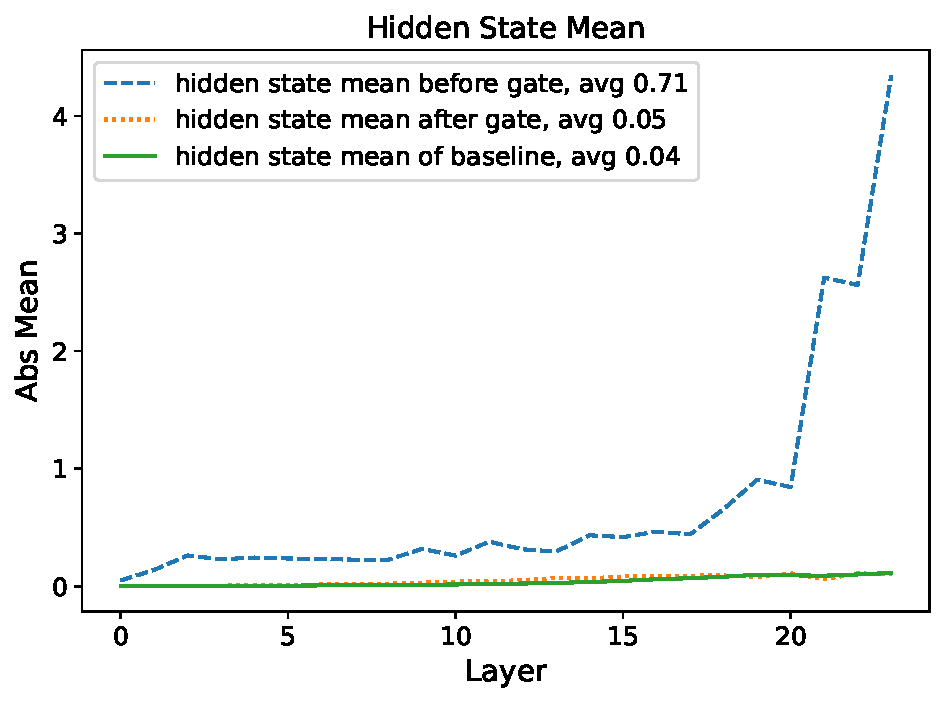
\includegraphics[width=0.5\textwidth]{imgs/hidden_states_mean.pdf}
    }
\vskip  -0.1in
  \caption{\footnotesize 
  门控前后平均绝对值。基线与门控后的数值相近。
  }
  \label{fig:gate_hidden_states}
  \end{center}
  \vskip  -0.1in
\end{figure*}


本节分析门控分数稀疏性对注意力输出的影响。
首先，我们考察隐藏状态在门控前后 SDPA 输出的均值。
具体地，我们计算每层在 $G_1$ 前后 $Y$ 与 $Y'$ 的平均绝对值，如图~\ref{fig:gate_hidden_states} 所示，并加入无门控的基线结果对比。
结果表明：(1) 门控后隐藏状态均值从 0.71 降至 0.05，对应门控分数整体较小；(2) 门控后的隐藏状态与基线非常接近，说明门控可能与 attention sink 起到类似的过滤无关信息的作用。



\begin{figure*}[ht]
    \vskip -0.05in  \begin{center}
    \centerline{
    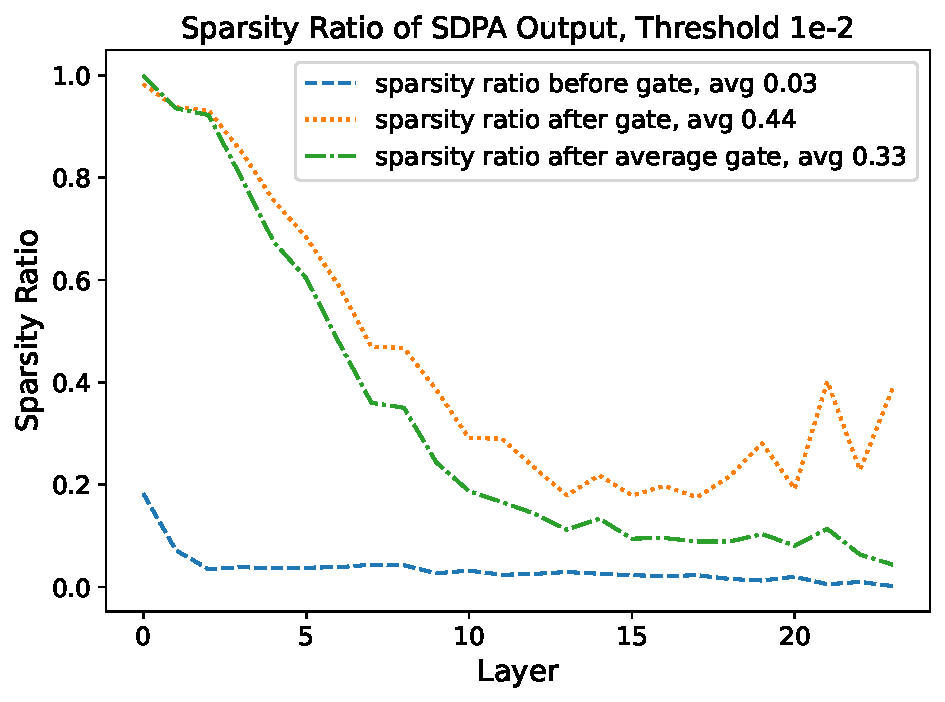
\includegraphics[width=0.45\textwidth]{imgs/sparsity_1e-2.pdf}
    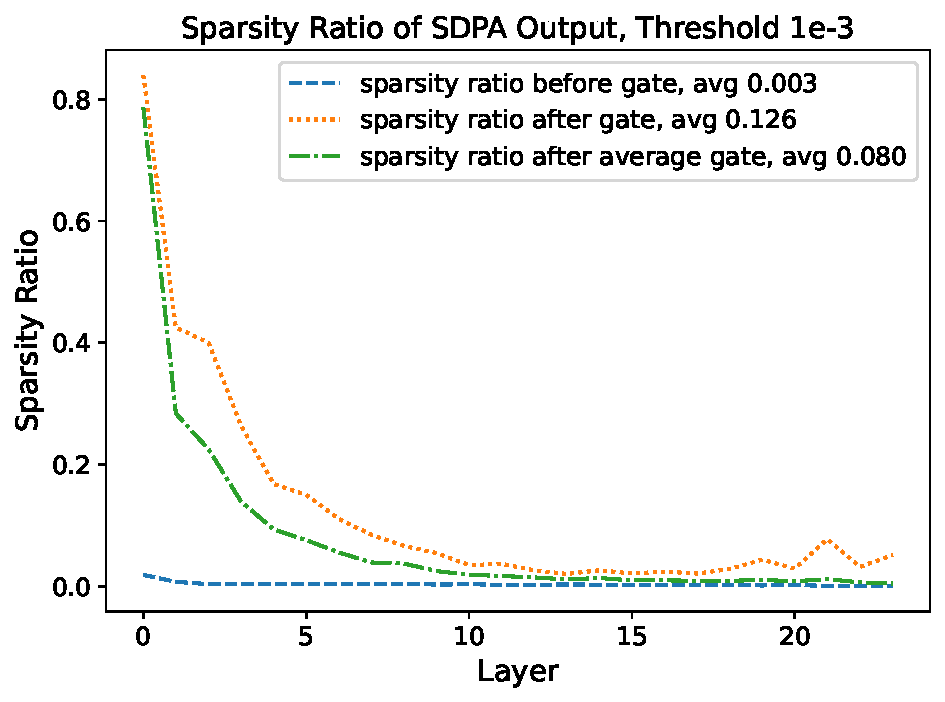
\includegraphics[width=0.45\textwidth]{imgs/sparsity_1e-3.pdf}
    }
\vskip  -0.1in
  \caption{\footnotesize 
  门控后 SDPA 输出低于阈值的比例（左：1e-2，右：1e-3）。同时给出将平均门控分数与门控前隐藏状态相乘得到的稀疏度。
  }
  \label{fig:sparsity_threshold}
  \end{center}
  \vskip  -0.1in
\end{figure*}


我们进一步分析门控前后隐藏状态低于不同阈值的比例，如图~\ref{fig:sparsity_threshold} 所示。
结果显示：(1) 门控后隐藏状态在各阈值下稀疏性显著提高。
由于平均门控分数已很小，将隐藏状态乘以小数会自然使部分数值低于阈值。
因此，我们将门控前隐藏状态乘以平均门控分数，发现稀疏性提升小于原始门控。
这表明稀疏的门控分数会增强隐藏状态的稀疏性。

\subsection{分层大幅激活与 Attention Sink}
\label{app:massive-sink}

本节比较并分析模型中大幅激活与 attention sink（首 token 的注意力分数）的存在情况。结果如下：

对于基线（第 1 行），第 6 层 FFN 的输出包含大幅激活，随后被加入残差流，使得较大的激活在后续层残差中持续存在。相应地，从第 6 层开始出现明显的 attention sink 现象。
在 SDPA 输出上施加门控（第 2 行）后，网络早期层的输出整体较小，大幅激活随层深逐步增长。
% This behavior aligns with the potential issue in pre-norm architectures where hidden states may grow excessively large when training very deep networks.
值得注意的是，网络各层均未观察到明显的 attention sink 现象。

仅在 value 层施加门控（第 3 行）时，模型的大幅激活与第 2 行类似。
但仍保留一定程度的 attention sink 现象，说明大幅激活并非 attention sink 出现的必要条件。
当对不同头强制共享门控分数（第 4 行）或修改门控的激活函数以抑制稀疏性（第 5 行）时，门控引入的稀疏性降低。在这些情况下，大幅激活与 attention sink 都与基线相当。

这些观察表明，在注意力机制中引入足够的稀疏性可能有助于缓解大幅激活的出现。但仍需进一步研究稀疏性、大幅激活与 attention sink 之间的相互作用，特别是在扩展到更深、更大模型的场景下。

\begin{figure*}[ht]
    \vskip -0.1in  \begin{center}
    \centerline{
    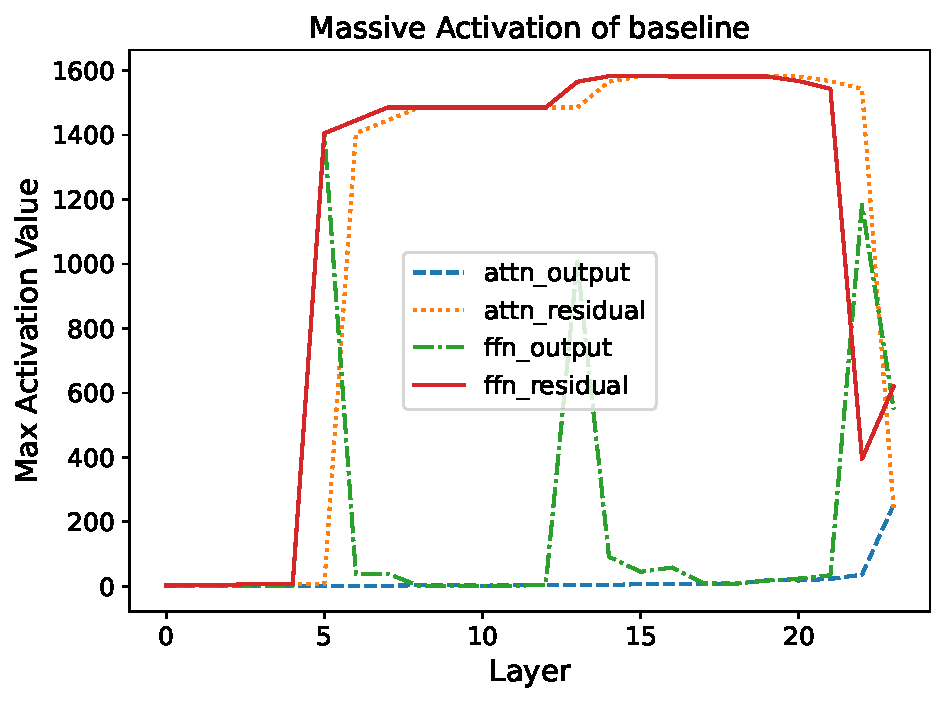
\includegraphics[width=0.37\textwidth]{imgs/baseline_massive_activation.pdf}
    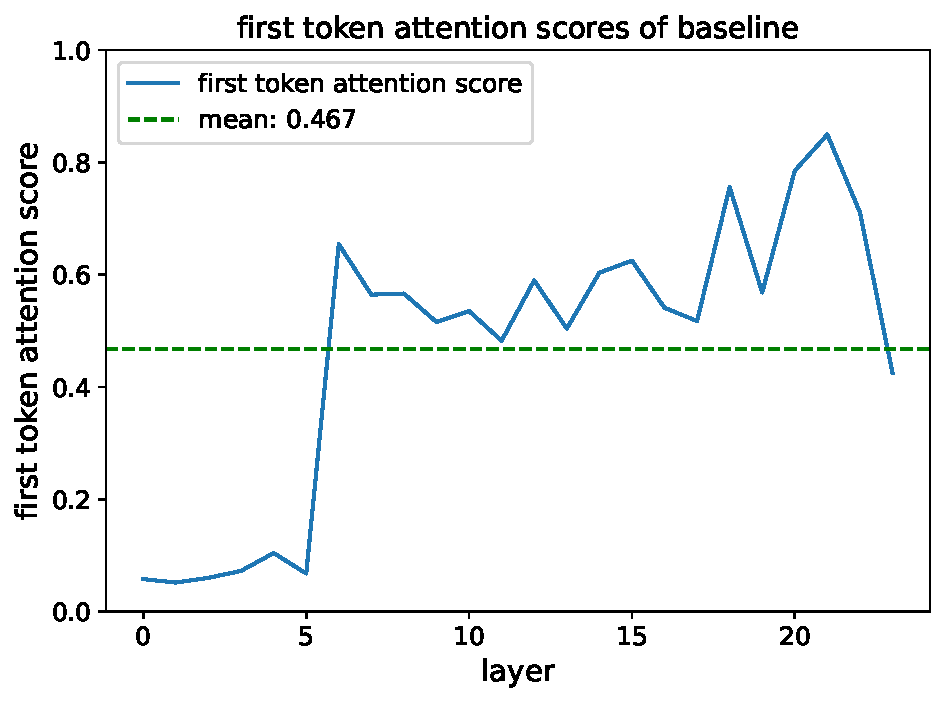
\includegraphics[width=0.37\textwidth]{imgs/baseline_first_token_scores.pdf}}
    \centerline{
    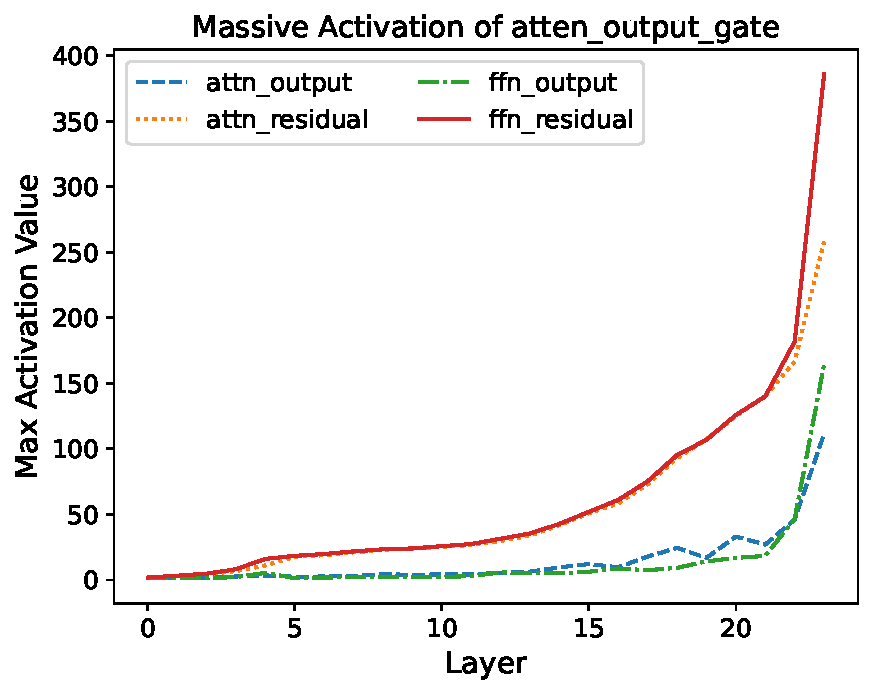
\includegraphics[width=0.37\textwidth]{imgs/atten_output_gate_massive_activation.pdf}
    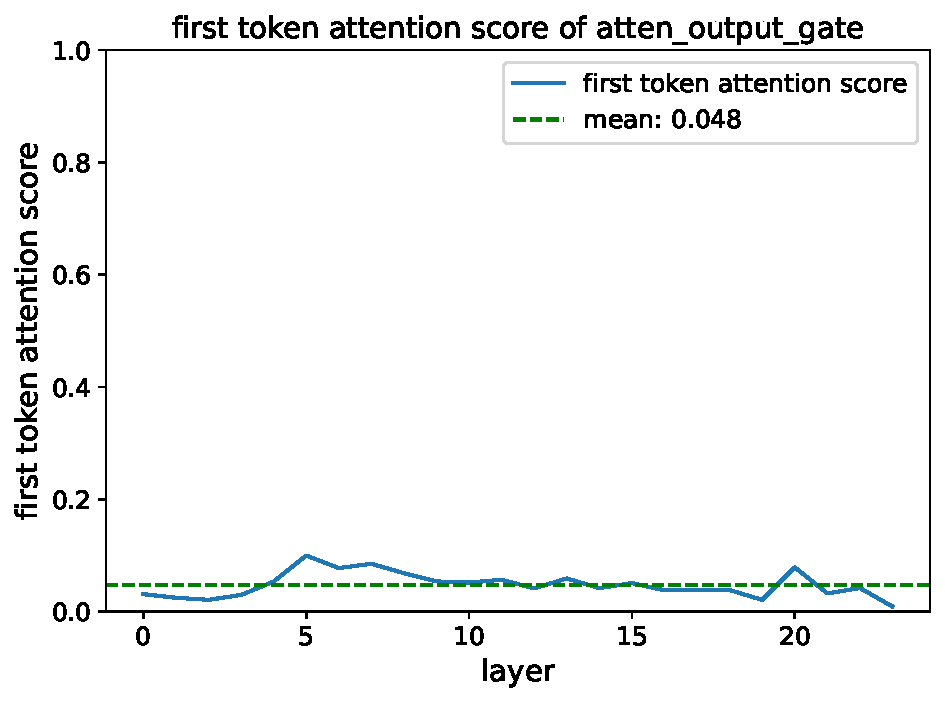
\includegraphics[width=0.37\textwidth]{imgs/atten_output_gate_first_token_scores.pdf}}
    \centerline{
    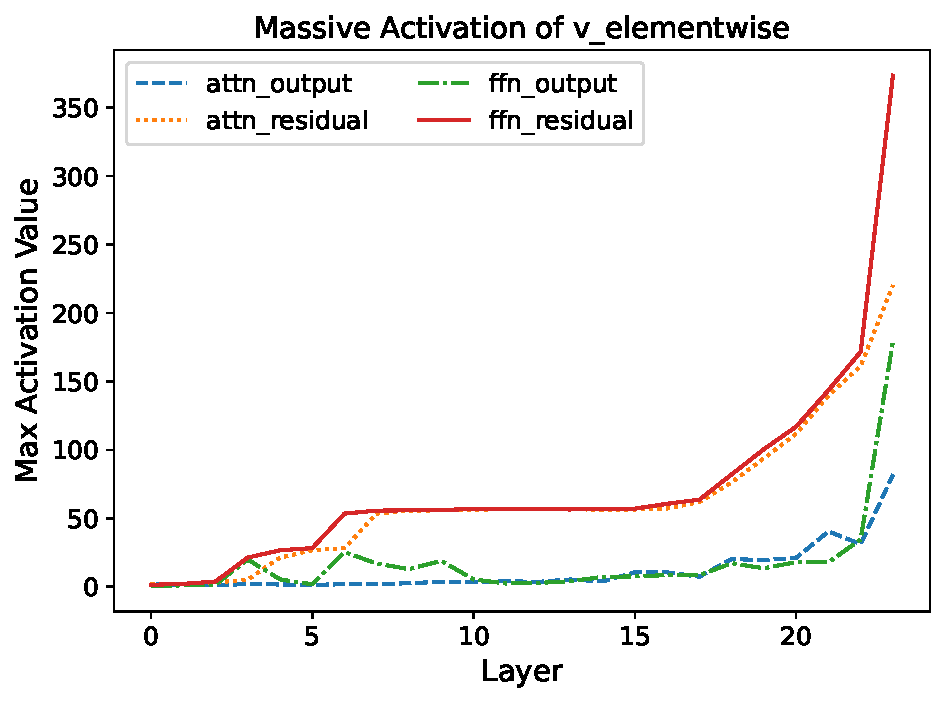
\includegraphics[width=0.37\textwidth]{imgs/v_elementwise_massive_activation.pdf}
    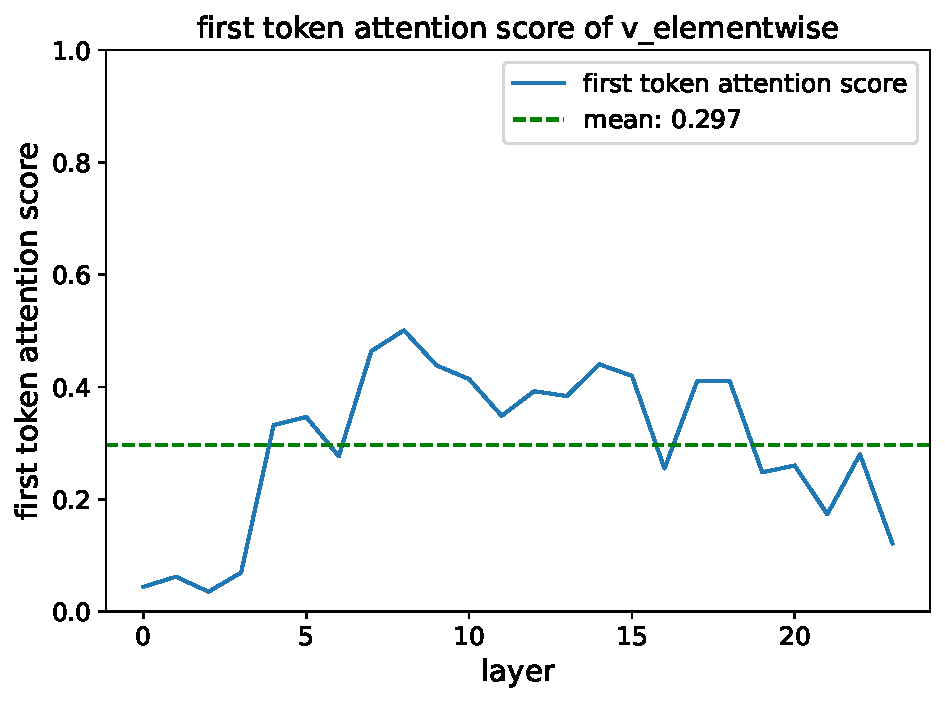
\includegraphics[width=0.37\textwidth]{imgs/v_elementwise_first_token_scores.pdf}
    }
    \centerline{
    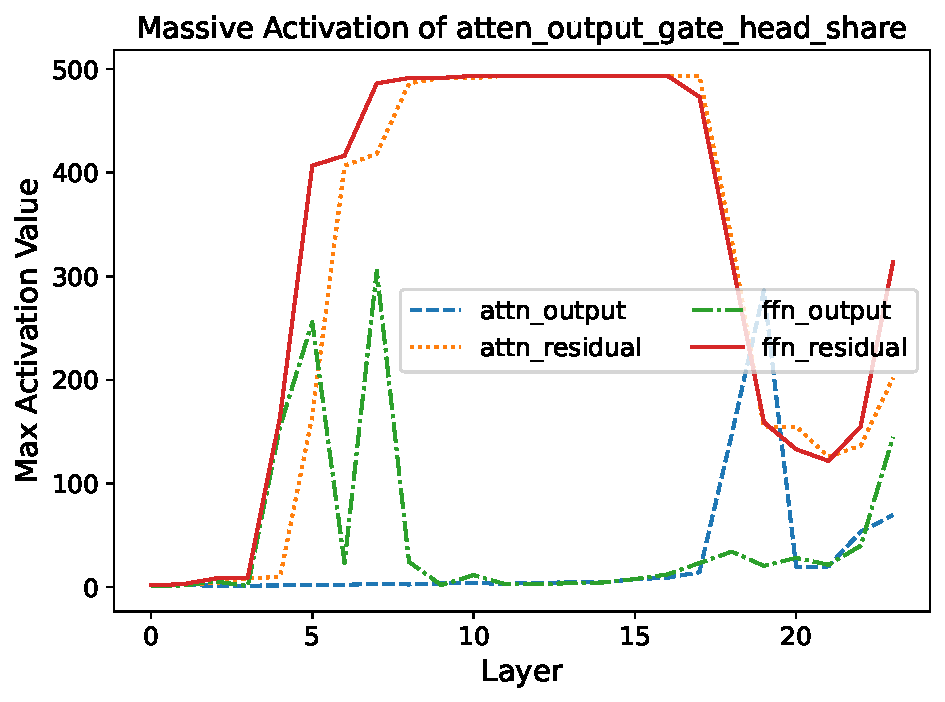
\includegraphics[width=0.37\textwidth]{imgs/atten_output_gate_head_share_massive_activation.pdf}
    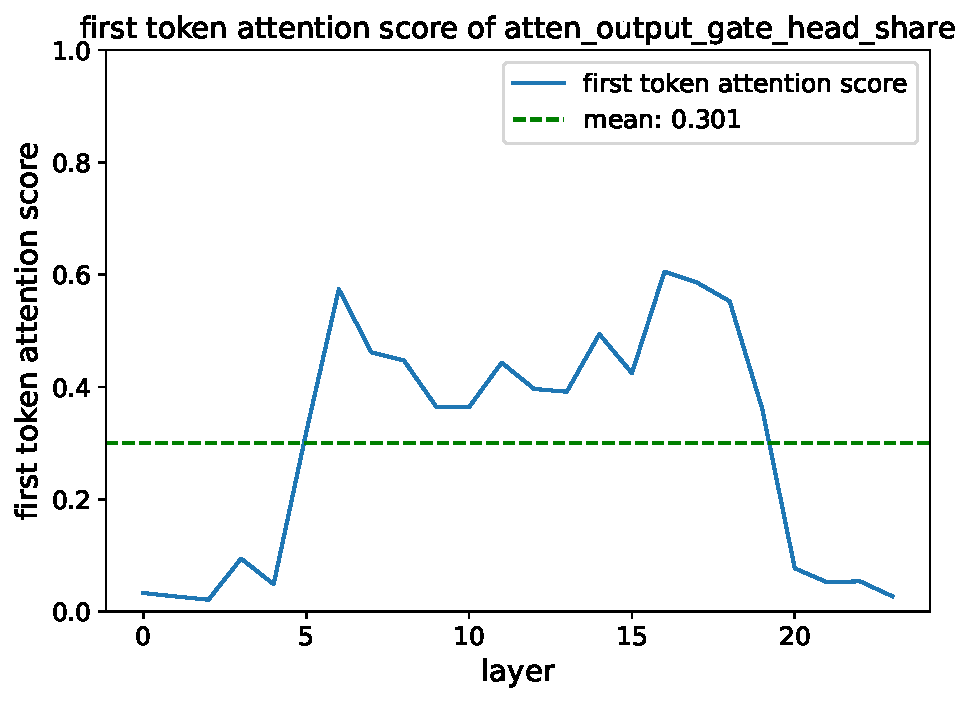
\includegraphics[width=0.37\textwidth]{imgs/atten_output_gate_head_share_first_token_scores.pdf}
    }
    \centerline{
    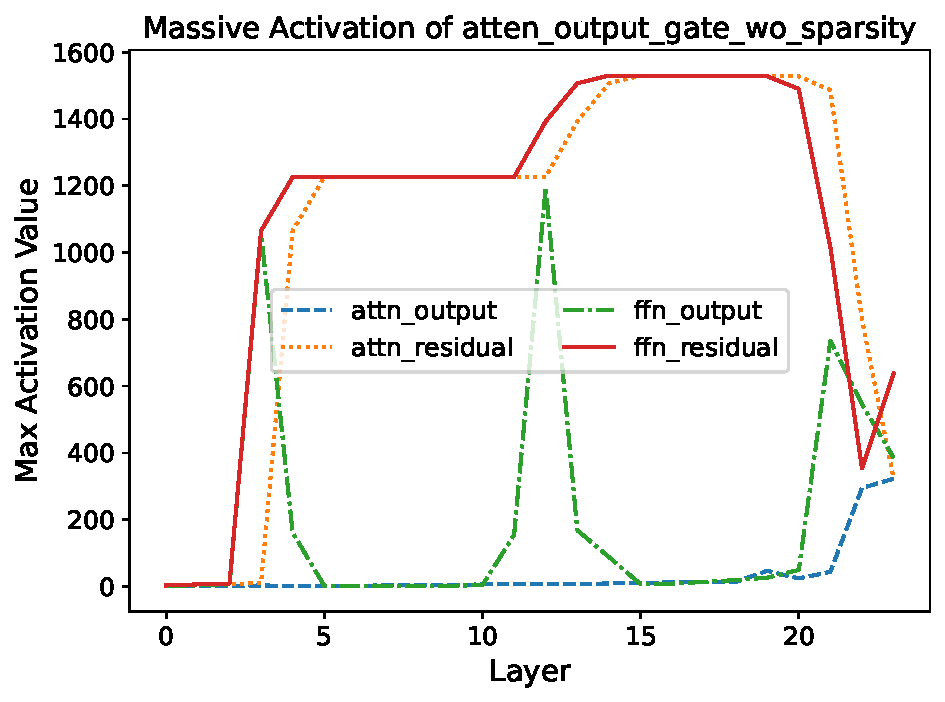
\includegraphics[width=0.37\textwidth]{imgs/atten_output_gate_wo_sparsity_massive_activation.pdf}
    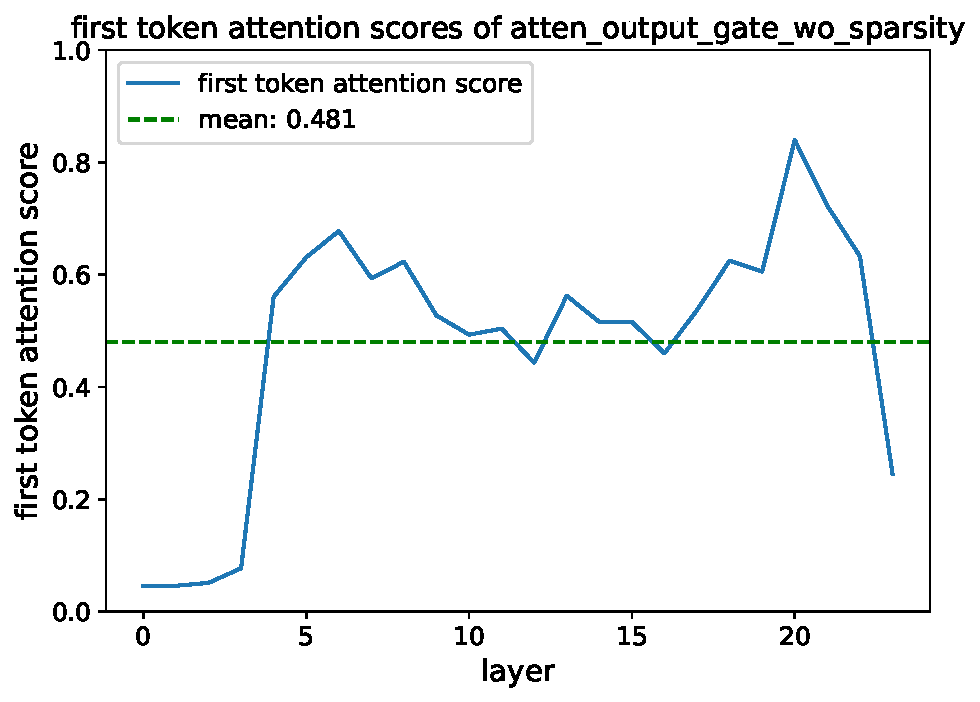
\includegraphics[width=0.37\textwidth]{imgs/atten_output_gate_wo_sparsity_first_token_scores.pdf}
    }
\vskip  -0.1in
  \caption{\footnotesize 
不同门控配置下的大幅激活与 attention sink 现象对比。
第 1 行（基线）：第 6 层后出现明显的大幅激活与 attention sink。
第 2 行（SDPA 门控）：激活减小且未观察到 attention sink。
第 3 行（Value 层门控）：与第 2 行激活相近但仍存在 attention sink。
第 4–5 行（跨头共享与 NS-sigmoid 降低稀疏性）：大幅激活与 attention sink 接近基线。
}\label{fig:layerwise_massive_activation_sinks}
  \end{center}
  \vskip  -0.3in
\end{figure*}

\subsection{分层门控分数的进一步分析}

本节在以 SDPA 输出门控为基线（第 1 行，逐元素/逐头）时，分析两种额外约束下的门控分数分布：(1) 跨不同头共享同一门控分数（第 2 行左）；(2) 限制门控分数的最小值（第 2 行右）。
当强制不同头共享门控分数时，多数层的门控分数会升高。
这表明不同头需要不同的稀疏性，强调了头特定门控机制的重要性。

\begin{figure*}[ht]
    \vskip -0.05in  \begin{center}
    \centerline{
    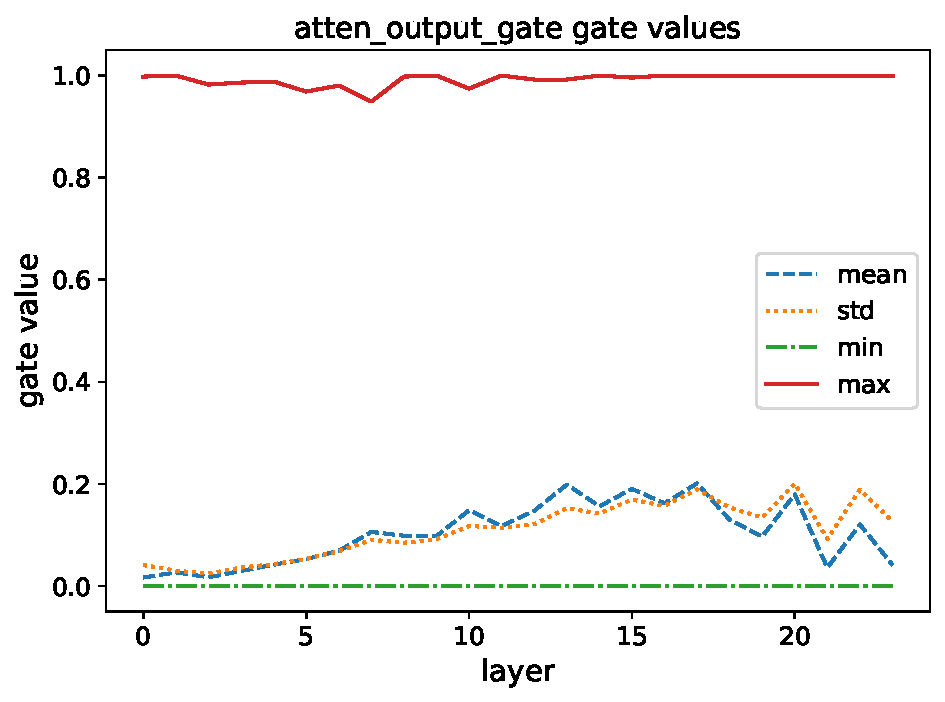
\includegraphics[width=0.45\textwidth]{imgs/atten_output_gate_gate_values.pdf}
    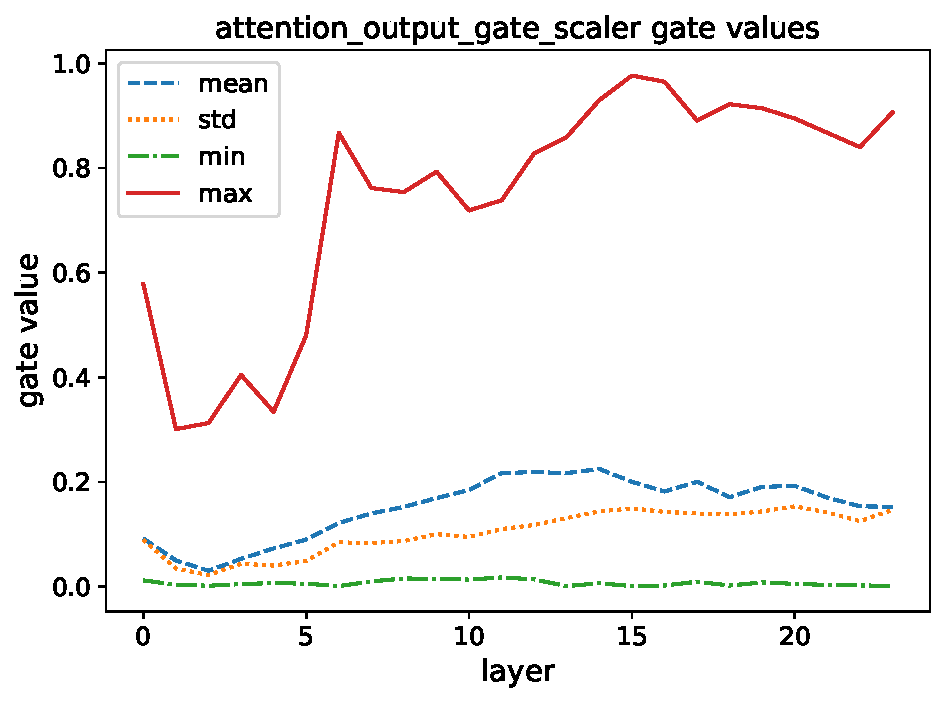
\includegraphics[width=0.45\textwidth]{imgs/attention_output_gate_scaler_gate_values.pdf}
    }
    \centerline{
    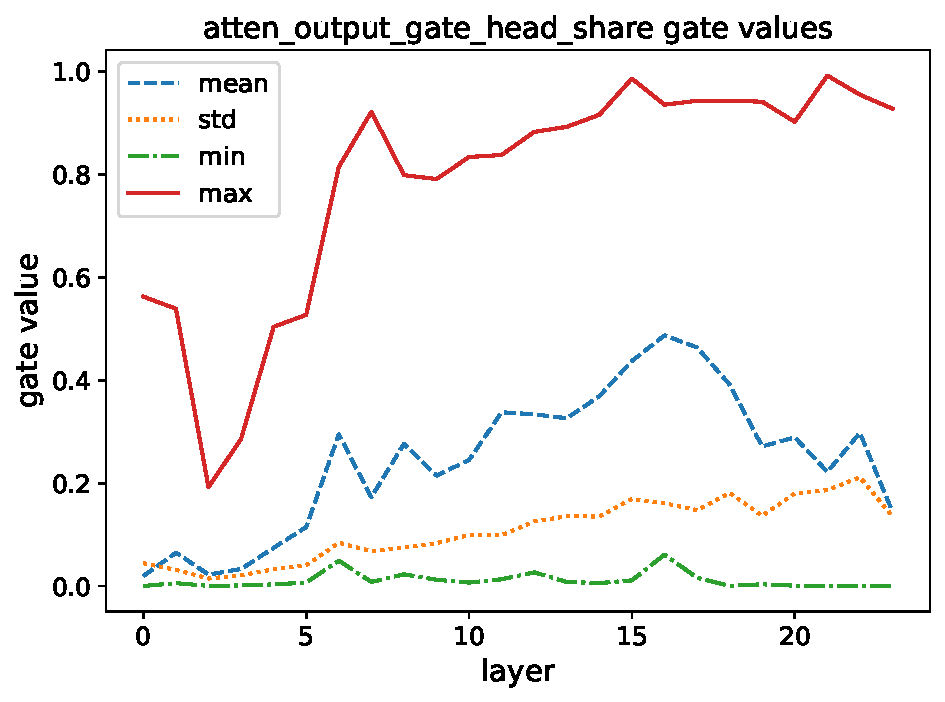
\includegraphics[width=0.45\textwidth]{imgs/atten_output_gate_head_share_gate_values.pdf}
    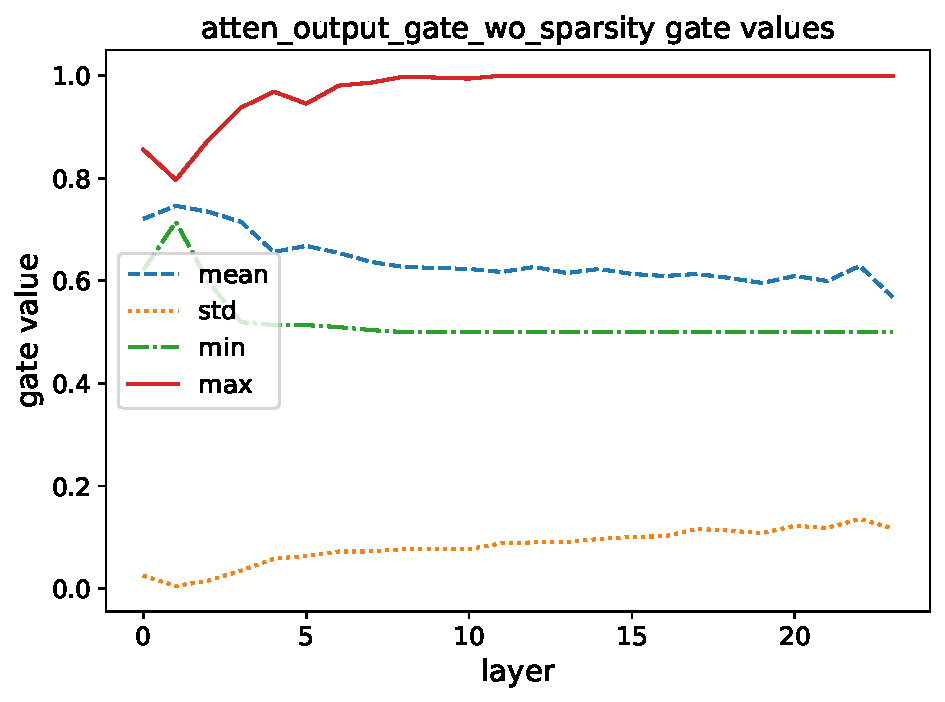
\includegraphics[width=0.45\textwidth]{imgs/atten_output_gate_wo_sparsity_gate_values.pdf}}
\vskip  -0.1in
  \caption{\footnotesize 
  不同约束下 SDPA 输出门控变体的门控分数分布。
  }
  \label{fig:layerwise_gate_values}
  \end{center}
  \vskip  -0.3in
\end{figure*}

\subsection{稳定训练的其他尝试}

我们观察到，加入 sandwich normalization~\citep{ding2021cogview} 与门控机制都能消除大幅激活并提升训练稳定性。
这促使我们探索更简单的方法是否可以抑制残差中的大激活。
具体而言，我们在注意力与 FFN 层输出进入残差连接之前引入裁剪操作，将其取值限制在 (-clip, clip) 范围内。
然而，无论 clip 设为 300 还是 100，在学习率 8e-3 下模型仍出现收敛问题。
这表明 pre-norm 模型训练的不稳定性并非仅由残差中的大激活造成。
任何层产生的大输出都可能导致稳定性问题，提示需要进一步研究训练不稳定的根因。

\end{document}
